\documentclass[12pt,a4paper]{article}

%% --- Packages ---
\usepackage[top=2.5cm,bottom=2.5cm,left=2.5cm,right=2.5cm]{geometry}
\usepackage[utf8]{inputenc}
\usepackage[T1]{fontenc}
\usepackage{lmodern}
\usepackage{graphicx}
\graphicspath{{./}}
\usepackage{booktabs}
\usepackage[hidelinks]{hyperref}
\usepackage{fancyhdr}
\usepackage{amsmath}
\usepackage{amssymb}
\usepackage{float}
\usepackage{tikz}
\usetikzlibrary{shapes.geometric,arrows.meta,positioning,backgrounds,fit}
\usepackage{array}
\usepackage{tabularx}
\usepackage{longtable}
\usepackage{multirow}
\usepackage{caption}
\usepackage{subcaption}
\usepackage{lastpage}
\usepackage{microtype}
\usepackage{parskip}
\usepackage{setspace}
\usepackage{xcolor}

%% --- Page style ---
\setlength{\headheight}{14.5pt}
\pagestyle{fancy}
\fancyhf{}
\lhead{Usama Asif}
\rhead{a1917716}
\cfoot{Page \thepage\ of \pageref{LastPage}}
\renewcommand{\headrulewidth}{0.4pt}

\fancypagestyle{plain}{%
  \fancyhf{}
  \renewcommand{\headrulewidth}{0pt}
}

\setlength{\parindent}{0pt}
\setlength{\parskip}{6pt}

%% ================================================================
\begin{document}

%% ===================== TITLE PAGE =====================
\begin{titlepage}
\centering
\vspace*{1.5cm}

{\LARGE\bfseries Analysing BBL Data to Understand the\\[8pt]
Impact of Home Advantage on the Game\\[6pt]
Final Report\par}

\vspace{2cm}

{\large Usama Asif\\[4pt]
\textbf{a1917716}\par}

\vspace{1.2cm}

{\large May 2026\par}

\vspace{1.8cm}

{\normalsize
Report submitted for \textbf{Data Science Project B} at the\\[4pt]
School of Mathematical Sciences, Adelaide University\par}

\vspace{1.5cm}


\includegraphics[width=0.45\textwidth]{Adelaide-University-Logo-New.png}\par

\vfill

\begin{flushleft}
Project Area: \textbf{Data Science for Cricket}\\[6pt]
Project Supervisor: \textbf{Mikaela Fudolig}
\end{flushleft}

\vspace{0.8cm}

{\small\itshape
In submitting this work I am indicating that I have read the University's Academic
Integrity Policy. I declare that all material in this assessment is my own work except
where there is clear acknowledgement and reference to the work of others.

\vspace{0.4cm}

I give permission for this work to be reproduced and submitted to other academic
staff for educational purposes.

\vspace{0.4cm}

I give permission for this work to be reproduced and provided to future
students as an exemplar report.\par}

\end{titlepage}

%% ===================== ABSTRACT =====================
\newpage
\begin{abstract}
\noindent
This report extends Project~A's analysis of home-ground advantage in the Big Bash League
(BBL) with a rebuilt modelling framework. The dataset uses \textbf{two rows per match}, one
per team, per the instructor's specification, with \texttt{match\_id} as a random intercept
to handle within-match correlation. Feature engineering uses strictly historical, lag-based
metrics; bowling team attribution and batting average are recomputed from scratch. Five
models are fitted and compared: a baseline logistic regression on home status only~(M1), a
full logistic regression on ten predictors~(M2), a LASSO interaction model~(M3), a Bayesian
GLMM~(M4), and \texttt{lme4}'s \texttt{glmer} via \texttt{rpy2}~(M5). Home-ground status is
a statistically significant predictor in isolation (M1:~OR\,=\,1.36, $p = 0.008$) and after
controlling for all predictors (M2:~OR\,=\,1.39, $p = 0.005$; M5:~OR\,=\,1.40,
$p = 0.004$). Recent form and head-to-head win rate are also significant. Familiarity metrics
drop out once the leakage correction is applied. A parallel extended analysis tests toss
outcomes, first-innings scoring, season trends, franchise effects, DRS umpiring, home bowling
defence, and first-six-over performance.
\end{abstract}

\newpage
\tableofcontents
\newpage

%% ===================== 1. INTRODUCTION =====================
\section{Introduction}

This report analyses fourteen seasons of Big Bash League (BBL) data, from 2011/12 to
2024/25. The BBL is Australia's premier Twenty20 cricket competition, contested annually
by eight city-based franchises. Attendances have varied substantially over time, peaking
above 30,000 per match in 2016/17, falling during the COVID period, and recovering in
recent seasons. The league draws a growing international broadcast audience. For franchise
management, coaches, and analysts, understanding what drives match outcomes matters: it informs venue strategy, squad selection,
travel scheduling, and pre-match forecasting.

Home-ground advantage is documented across professional sports~[12], but its drivers in the
BBL remain untested at the player-metric level. In T20 cricket, pitch conditions, boundary
dimensions, crowd pressure, and travel fatigue all run together. Separating their contributions requires a framework that controls for team quality while
isolating the venue effect.

Prior cricket modelling covers toss effects~[10], team ratings~[1], and in-game win
probability~[2], but few studies isolate home advantage using historical venue-level features
and mixed-effects models. Small per-venue samples, player transfers across franchises, and the
confounding effect of team quality make isolation difficult in T20 cricket. Pitch familiarity
and travel explain home advantage in English one-day cricket~[8]; no equivalent study exists
for the BBL.

Project~A established a logistic regression baseline using home status, toss outcome, recent
form, and player-venue familiarity. Project~B responds to instructor feedback by adopting the
two-rows-per-match structure, adding mixed-effects models, and comparing five models to
identify which predictors actually drive BBL outcomes.

\subsection*{Research Objectives}

\begin{enumerate}
  \item Quantify the raw home advantage in BBL across the 14 seasons available in the dataset (2011/12 to 2024/25).
  \item Test whether home advantage persists after controlling for team form, head-to-head
    history, toss outcome, and venue familiarity metrics.
  \item Determine whether player- and venue-level familiarity explains the home advantage
    signal, or whether it remains an independent predictor after controlling for those metrics.
  \item Assess robustness across venue types, COVID-era scheduling disruptions, and extended
    match phases including first-six-over performance, first-innings scoring, and DRS umpiring.
\end{enumerate}

%% ===================== 2. BACKGROUND =====================
\section{Background}

\subsection{Literature Review}

Home teams win more often across professional sports, with effect sizes varying by league
structure, travel load, and crowd size~[5]. Courneya and Carron~[12] identify three
mechanisms: venue familiarity, crowd effects on opponents and officials, and travel fatigue
in away teams. Pollard~[13] confirmed the same effects across different sports, with venue familiarity and
travel distance the most consistent predictors.

In cricket, pitch characteristics, boundary shape, wind direction, and lighting all shape
batting and bowling performance~[8]. Players who have performed at a ground accumulate
venue-specific knowledge that career averages miss. Adelaide Oval's short straight boundaries
and slow pitch play differently from the Gabba's pace-friendly surface. Crowd attendance may
also bias umpiring decisions~[6]; the BBL's DRS system, available from 2022/23 onward, lets
us test this directly.

English one-day cricket research attributes home advantage to pitch knowledge and travel
rather than crowd size~[8]. Win probability models for one-day internationals~[2] and team
rating models in test cricket~[1] did not isolate venue familiarity as a predictor. T20
analyses show mixed evidence on home advantage and toss effects~[10]. Swartz and Arce~[14] found significant but heterogeneous home advantage effects across
cricket teams and venues, consistent with the BBL pattern here.

Mixed-effects models suit grouped observations. Each match contributes two correlated rows
because exactly one team wins; random intercepts for match and team follow standard practice
in clustered sports data~[15] and give a more defensible test of the home advantage
coefficient than a pooled logistic regression.

\subsection{Improvements Since Project~A}

Project~B makes seven improvements since Project~A, in response to instructor feedback:

\begin{enumerate}
  \item \textbf{Two-rows-per-match structure adopted.} Project~A used one row per match (home
    team perspective only). Each match now contributes two rows, one per team, so that
    \texttt{is\_home} is a proper within-match predictor. \texttt{match\_id} is included as
    a random intercept in M4 and M5.

  \item \textbf{Five-model suite.} The suite fits and compares a baseline (M1), full logistic
    (M2), LASSO interaction (M3), Bayesian GLMM (M4), and \texttt{lme4} \texttt{glmer} (M5).

  \item \textbf{Full coefficient interpretation.} All table outputs (coefficients, standard
    errors, $p$-values, and odds ratios) are explicitly interpreted in
    Section~\ref{sec:results}.

  \item \textbf{Random effects implemented.} M4 and M5 include
    \texttt{(1|team) + (1|match\_id)} random intercepts as specified by the instructor.

  \item \textbf{DRS umpiring analysis added.} An umpiring bias analysis using ball-by-ball DRS
    data tests whether umpires systematically favour home teams in review decisions.

  \item \textbf{CSV reproducibility pipeline.} Intermediate CSV files are exported at every
    transformation step, enabling full reproduction from raw JSON to final model outputs.

  \item \textbf{Revised visualisation.} The single home-win bar chart from Project~A is
    replaced with a grouped home-vs-away chart per franchise.
\end{enumerate}

%% ===================== 3. METHODS =====================
\section{Methods}

All code runs in Python. The modelling pipeline is in \texttt{BBL\_Home\_Advantage\_Model.ipynb};
extended analyses are in \texttt{BBL\_Extended\_Analysis.ipynb}. Code is available at:
\url{https://github.com/UsamaAsif10/BBL-Analysis-Project-Part-B}.

Figure~\ref{fig:pipeline} shows the project pipeline.

\begin{figure}[H]
\centering
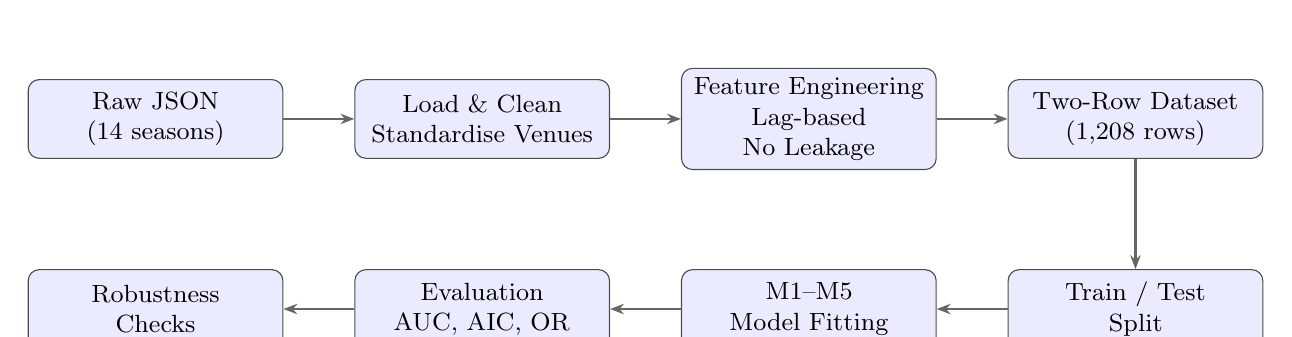
\begin{tikzpicture}[
  node distance=0.55cm and 0.9cm,
  box/.style={rectangle, rounded corners=4pt, draw=black!70, fill=blue!8,
              text width=3.0cm, align=center, minimum height=1.0cm, font=\small},
  arrow/.style={-{Stealth[length=5pt]}, thick, draw=black!60},
]
%% Top row: data pipeline
\node[box] (json)  {Raw JSON\\(14 seasons)};
\node[box, right=of json]  (clean) {Load \& Clean\\Standardise Venues};
\node[box, right=of clean] (feat)  {Feature Engineering\\Lag-based\\No Leakage};
\node[box, right=of feat]  (ds)    {Two-Row Dataset\\(1{,}208 rows)};

%% Bottom row: modelling pipeline
\node[box, below=1.4cm of ds]      (split)   {Train / Test\\Split};
\node[box, left=of split]          (models)  {M1--M5\\Model Fitting};
\node[box, left=of models]         (eval)    {Evaluation\\AUC, AIC, OR};
\node[box, left=of eval]           (robust)  {Robustness\\Checks};

%% Top row arrows
\draw[arrow] (json)  -- (clean);
\draw[arrow] (clean) -- (feat);
\draw[arrow] (feat)  -- (ds);
\draw[arrow] (ds)    -- (split);

%% Bottom row arrows
\draw[arrow] (split)  -- (models);
\draw[arrow] (models) -- (eval);
\draw[arrow] (eval)   -- (robust);
\end{tikzpicture}
\caption{Project pipeline: from raw JSON data to robustness-checked model estimates.}
\label{fig:pipeline}
\end{figure}

\subsection{Data}

The dataset covers 14 BBL seasons (2011/12 to 2024/25) as JSON files, loaded recursively with
UTF-8 and Latin-1 fallbacks. A mapping dictionary standardised venue names; venue/franchise heuristics assigned home
teams. Excluding no-result, abandoned, tied, and missing-winner matches left \textbf{604
decisive matches} and \textbf{143,323 delivery records}.

\textbf{CSV exports:} \texttt{cleaned\_match\_data.csv}, \texttt{cleaned\_ball\_by\_ball\_data.csv}.

I computed descriptive statistics per team per season: home and away win rates, and
\[
  \text{HAI}_{t,s} = \text{HomeWinRate}_{t,s} - \text{AwayWinRate}_{t,s}.
\]
A positive HAI indicates home benefit; a negative HAI indicates better away performance.

\textbf{CSV exports:} \texttt{season\_stats.csv}, \texttt{home\_ground\_stats.csv},
\texttt{home\_away\_win\_probability.csv}, \texttt{home\_advantage\_index.csv}.

\subsection{Data Structure and Feature Engineering}

Each match contributes two rows, one per team, with fields \texttt{match\_id},
\texttt{team}, \texttt{opponent}, \texttt{venue}, \texttt{is\_home}, \texttt{win}, and ten
predictors (Table~\ref{tab:predictors}). Total: \textbf{1,208 rows} from 604 matches.

Every predictor uses \texttt{shift(1).expanding()} so only prior-match data feeds into each
row. For comparability across seasons, this report defines a common
\textit{first-six-over phase} rather than relying on season-specific powerplay rules (BBL
powerplay regulations changed with the introduction of the Power Surge). \texttt{h2h\_win\_rate}
uses Bayesian shrinkage to stabilise head-to-head pairs with few encounters:
\[
  \hat{\pi} = \frac{\text{wins} + k/2}{\text{games} + k}, \quad k = 5.
\]

\textbf{CSV exports:} \texttt{model\_df\_step1\_tworow.csv}; \texttt{model\_df\_v2.csv}
(1,208 rows, 10 predictors, zero nulls).

\begin{table}[H]
\centering
\caption{Predictor variables in the modelling dataset.}
\label{tab:predictors}
\small
\begin{tabularx}{\textwidth}{lXl}
\toprule
\textbf{Predictor} & \textbf{Description} & \textbf{Direction} \\
\midrule
\texttt{is\_home} & 1 if this team is the home team & Positive \\
\texttt{toss\_win} & 1 if this team won the toss & Positive \\
\texttt{toss\_bat} & 1 if toss winner elected to bat & Uncertain \\
\texttt{recent\_form\_5} & Win proportion of last 5 matches (lagged) & Positive \\
\texttt{h2h\_win\_rate} & Head-to-head win rate vs opponent (Bayesian, $k=5$) & Positive \\
\texttt{pp\_rr\_lag5} & Avg.\ first-six-over run rate over last 5 matches (lagged) & Positive \\
\texttt{team\_bat\_sr\_familiarity} & Team batting strike rate at venue (historical) & Positive \\
\texttt{team\_bat\_avg\_familiarity} & Team batting average at venue (historical) & Positive \\
\texttt{team\_bowl\_eco\_familiarity} & Negative of team bowling economy at venue & Positive \\
\texttt{team\_bowl\_sr\_familiarity} & Negative of team bowling strike rate at venue & Positive \\
\bottomrule
\end{tabularx}
\end{table}

\subsection{Models}

Five models are fitted to the two-row dataset:

\textbf{M1:} Baseline logistic regression, \texttt{win \textasciitilde\ is\_home}.
Establishes the unadjusted home advantage. Fitted with \texttt{method=`bfgs'}.

\textbf{M2:} Full logistic regression, All ten predictors. Primary inferential model.
Fitted with \texttt{method=`bfgs'}, \texttt{maxiter=300}.

\textbf{M3:} LASSO interaction model, $L_1$-penalised logistic regression~[11]
($C = 0.05$) applied to all 45 pairwise interactions; surviving terms re-fitted without
penalisation.

\textbf{M4:} Bayesian GLMM, \texttt{statsmodels.BinomialBayesMixedGLM} with fixed
effects as in M2 and \texttt{(1|team) + (1|match\_id)} random intercepts. Estimated via
variational Bayes.

\textbf{M5:} \texttt{lme4 glmer} via \texttt{rpy2}, Gold-standard mixed-effects
specification using R's \texttt{lme4}~[3] called directly from Python via \texttt{rpy2},
with \texttt{optimizer=`bobyqa'}.

\textbf{Train/test split.} Models were trained chronologically on matches before the 2023/24
season and evaluated on matches from 2023/24 onward. A chronological split was used rather
than a random split to better mimic future match prediction and reduce temporal leakage.
Predictive metrics (AUC, accuracy, ROC curve, confusion matrix) are reported on this
chronological holdout period (160 test rows). Coefficient tables are estimated on the
training set (1,048 rows). Some exported CSV files contain full-sample diagnostics
(e.g., \texttt{model\_comparison.csv} reports a full-sample AUC of 0.731), which will
differ from the holdout AUC of 0.676 quoted in the text.

%% ===================== 4. RESULTS AND DISCUSSION =====================
\section{Results and Discussion}
\label{sec:results}

\subsection{Descriptive Analysis: Home vs Away Win Rates}

Home teams won 54.8\% of matches, meaning away teams won 45.2\%. The $+4.8$~pp figure
refers to the gap above the 50\% baseline; the full home--away split is 54.8 versus 45.2
(a 9.6~pp difference between the two sides). Variation across franchises is large
(Figure~\ref{fig:homeaway}). Perth Scorchers (68.0\% home, 55.6\% away) and Sydney Sixers
(67.6\% home, 59.7\% away) are strong everywhere; their home win rates reflect team quality
as much as venue. Adelaide Strikers (gap\,=\,$+0.131$) and Hobart Hurricanes
(gap\,=\,$+0.119$) show the largest venue-specific edges. Brisbane Heat are the only
franchise with a negative gap ($-0.051$). Seven of eight franchises are positive.

\begin{figure}[H]
  \centering
  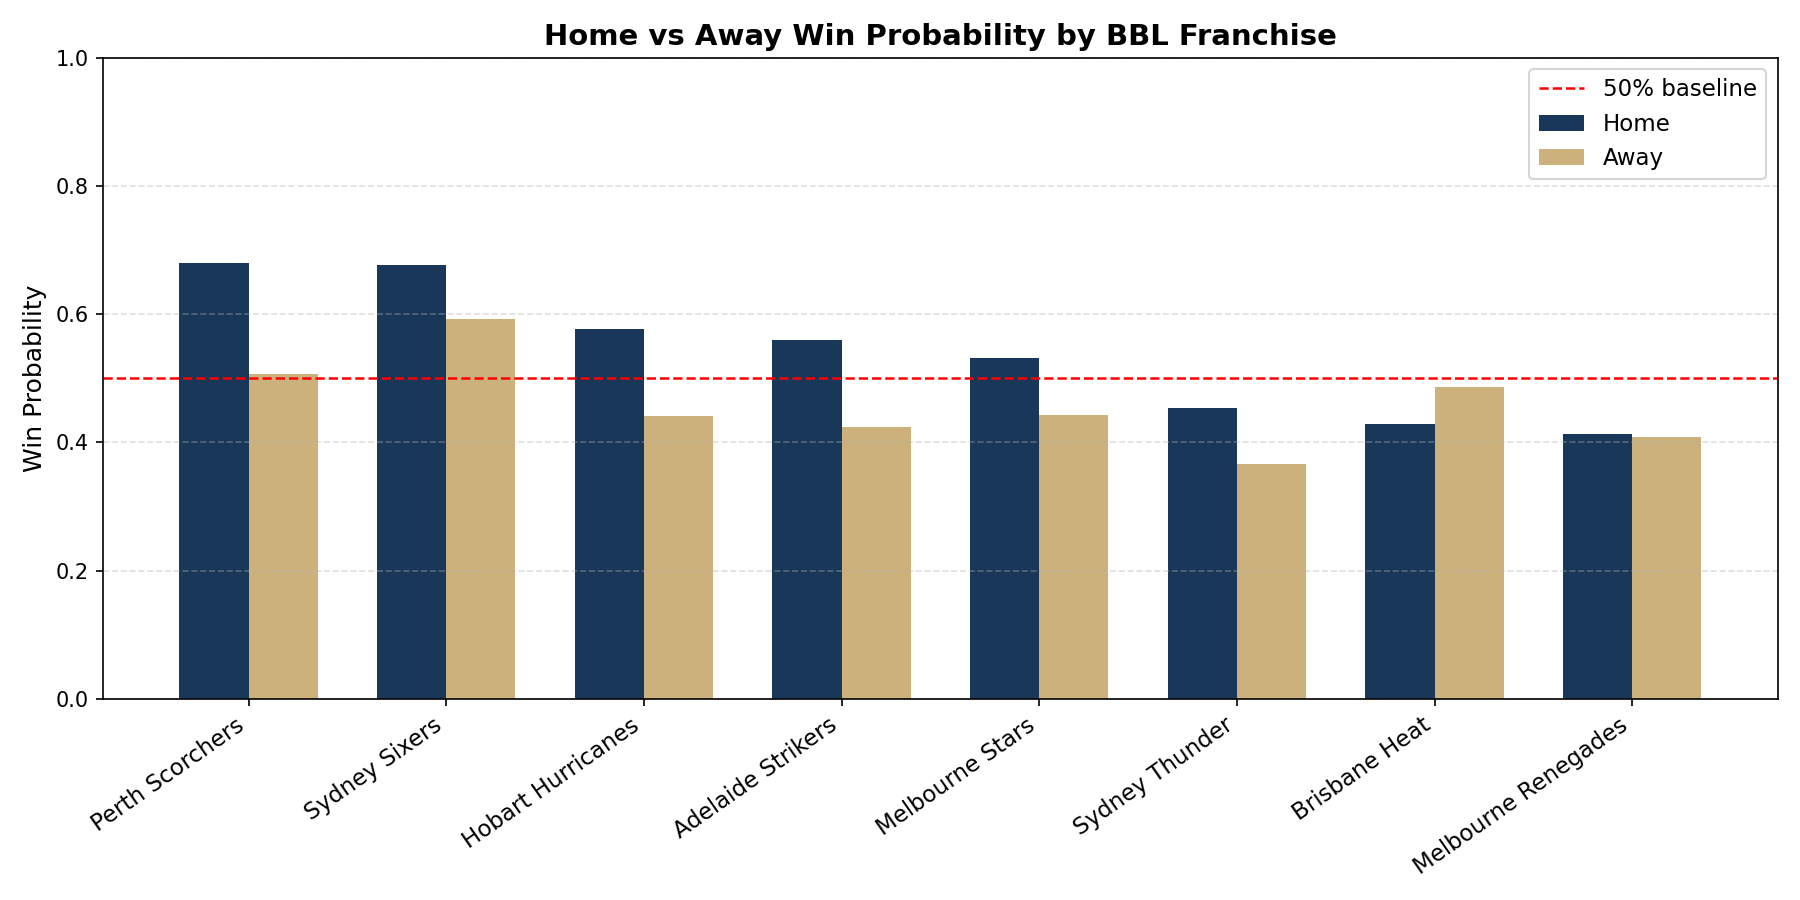
\includegraphics[width=0.88\textwidth]{home_away_chart.png}
  \caption{Home and away win rates per BBL franchise across all 14 seasons (2011/12--2024/25).}
  \label{fig:homeaway}
\end{figure}

\subsection{Predictive Models: M1 to M5}
\label{sec:models}

\subsubsection{M1: Baseline Model, Unadjusted Home Advantage}

M1 tests whether home teams win more often than chance, with no other controls. The model is:
\[
  \log\frac{P(\text{win})}{1 - P(\text{win})} = \beta_0 + \beta_1 \cdot \texttt{is\_home}
\]

\begin{table}[H]
\centering
\caption{M1 results --- Baseline logistic regression.}
\label{tab:m1}
\begin{tabular}{lcccc}
\toprule
\textbf{Parameter} & \textbf{Coef.} & \textbf{SE} & \textbf{$p$-value} & \textbf{OR} \\
\midrule
Intercept & $-0.143$ & $0.079$ & $0.070$ & --- \\
\texttt{is\_home} & $\mathbf{0.307}$ & $0.116$ & $\mathbf{0.008}$ & $\mathbf{1.36}$ \\
\bottomrule
\end{tabular}
\end{table}

The intercept converts to an away-team win probability of $\text{logistic}(-0.143) = 46.4\%$.
Adding the \texttt{is\_home} coefficient gives $\text{logistic}(-0.143 + 0.307) = 54.1\%$,
a $+7.7$~pp fitted probability difference relative to the away-team baseline (OR\,=\,1.36, $p = 0.008$). Pseudo~$R^2 = 0.004$ and
AUC\,=\,0.613: home status is statistically real but explains little variance alone.

M1 confirms home advantage exists; venue alone is a weak pre-match signal. Form and
head-to-head history carry more predictive weight. M2 tests whether home status survives
once those factors are controlled.

\subsubsection{M2: Full Model, Identifying the Drivers of Home Advantage}

M2 is the primary inferential model. It controls for all ten predictors simultaneously and
tests whether \texttt{is\_home} survives. The model is:
\begin{align*}
  \log\frac{P(\text{win})}{1 - P(\text{win})} &= \beta_0
    + \beta_1 \cdot \texttt{is\_home}
    + \beta_2 \cdot \texttt{toss\_win}
    + \beta_3 \cdot \texttt{toss\_bat} \\
  &\quad + \beta_4 \cdot \texttt{recent\_form\_5}
    + \beta_5 \cdot \texttt{h2h\_win\_rate}
    + \sum_{j=6}^{10} \beta_j x_j
\end{align*}
where $x_6, \ldots, x_{10}$ are the first-six-over run rate lag and four venue familiarity
metrics.

\begin{table}[H]
\centering
\caption{M2 results --- Full logistic regression (training set, $N = 1{,}048$).}
\label{tab:m2}
\small
\begin{tabular}{lccccc}
\toprule
\textbf{Predictor} & \textbf{Coef.} & \textbf{SE} & \textbf{$p$} & \textbf{OR} & \textbf{95\% CI} \\
\midrule
Intercept                           & $-2.985$ & $1.093$ & $0.006$ & ---     & --- \\
\textbf{\texttt{is\_home}}          & $\mathbf{0.330}$ & $0.118$ & $\mathbf{0.005}$ & $\mathbf{1.391}$ & $(1.103,\,1.755)$ \\
\texttt{toss\_win}                  & $0.210$  & $0.136$ & $0.123$ & $1.233$ & $(0.945,\,1.609)$ \\
\texttt{toss\_bat}                  & $-0.084$ & $0.168$ & $0.616$ & $0.919$ & $(0.662,\,1.277)$ \\
\textbf{\texttt{recent\_form\_5}}   & $\mathbf{0.503}$ & $0.250$ & $\mathbf{0.044}$ & $\mathbf{1.654}$ & $(1.013,\,2.700)$ \\
\textbf{\texttt{h2h\_win\_rate}}    & $\mathbf{1.276}$ & $0.559$ & $\mathbf{0.022}$ & $\mathbf{3.582}$ & $(1.197,\,10.714)$ \\
\texttt{pp\_rr\_lag5}               & $-0.023$ & $0.064$ & $0.714$ & $0.977$ & $(0.862,\,1.107)$ \\
\texttt{team\_bat\_sr\_familiarity} & $0.007$  & $0.008$ & $0.369$ & $1.007$ & $(0.991,\,1.024)$ \\
\texttt{team\_bat\_avg\_familiarity}& $-0.004$ & $0.007$ & $0.577$ & $0.996$ & $(0.983,\,1.010)$ \\
\texttt{team\_bowl\_eco\_familiarity}&$-0.140$ & $0.125$ & $0.262$ & $0.870$ & $(0.681,\,1.110)$ \\
\texttt{team\_bowl\_sr\_familiarity}& $-0.006$ & $0.013$ & $0.634$ & $0.994$ & $(0.969,\,1.019)$ \\
\bottomrule
\multicolumn{6}{l}{\small AUC\,=\,0.676 \quad Pseudo $R^2$\,=\,0.015 \quad AIC\,=\,1460.98}
\end{tabular}
\end{table}

\textbf{Predictor interpretation:}

\textbf{\texttt{is\_home}} (OR\,=\,1.391, $p = 0.005$): Home teams have 39\% higher odds
of winning the same match after controlling for form, head-to-head history, and venue
familiarity (CI: 1.10, 1.76). Home advantage is not absorbed by the other predictors.

\textbf{\texttt{toss\_win}} (OR\,=\,1.233, $p = 0.123$): Not significant. Winning the toss
adds no reliable win probability after controlling for team quality.

\textbf{\texttt{toss\_bat}} (OR\,=\,0.919, $p = 0.616$): Not significant. Choosing to bat
first is directionally negative, consistent with the T20 preference for chasing, but the
effect is not statistically reliable.

\textbf{\texttt{recent\_form\_5}} (OR\,=\,1.654, $p = 0.044$): Significant. Winning all
five recent matches gives $1.65\times$ higher win odds versus a team on a losing run.
Short-run form carries forward.

\textbf{\texttt{h2h\_win\_rate}} (OR\,=\,3.582, $p = 0.022$): The largest effect in the
model. A team with a dominant head-to-head record against a specific opponent has $3.6\times$
higher odds. The wide CI (1.20, 10.71) reflects thin historical encounter counts per pair.

\textbf{First-six-over and familiarity metrics} (all $p > 0.26$): None significant. Once built
from historical data only, these metrics carry no independent signal.

The core finding from M2 is that home advantage in the BBL remains an independent predictor
after controlling for team quality, form, head-to-head history, toss outcome, and venue
familiarity. A home team with average form, a neutral head-to-head record, and no particular
venue expertise still enters each match with 39\% higher odds of winning than their opponent. This has practical consequences for fixture scheduling, travel
planning, and any pre-match forecasting model that omits venue as a predictor.

\begin{figure}[H]
  \centering
  \begin{subfigure}[b]{0.47\textwidth}
    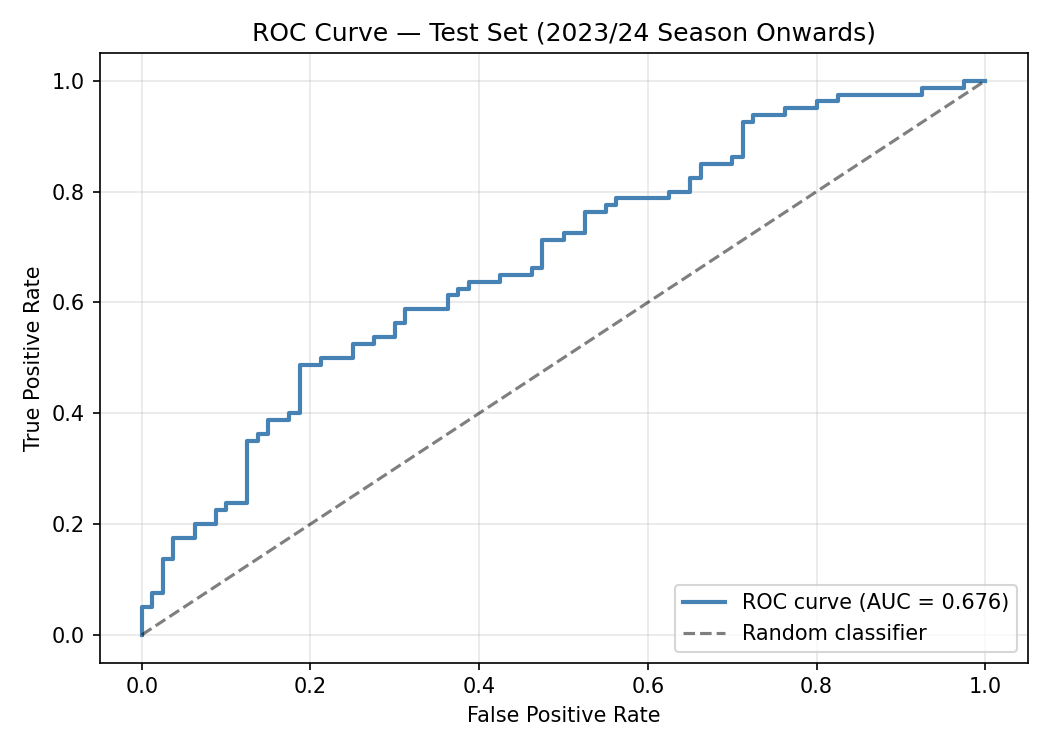
\includegraphics[width=\textwidth]{roc_curve.png}
    \caption{ROC curve (AUC\,=\,0.676).}
    \label{fig:roc}
  \end{subfigure}
  \hfill
  \begin{subfigure}[b]{0.47\textwidth}
    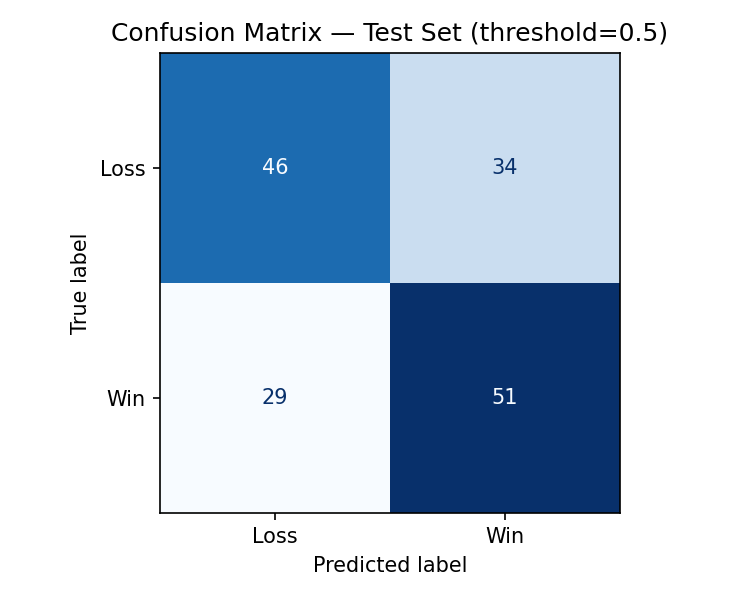
\includegraphics[width=\textwidth]{confusion_matrix.png}
    \caption{Confusion matrix.}
    \label{fig:cm}
  \end{subfigure}

  \vspace{0.5cm}

  \begin{subfigure}[b]{0.47\textwidth}
    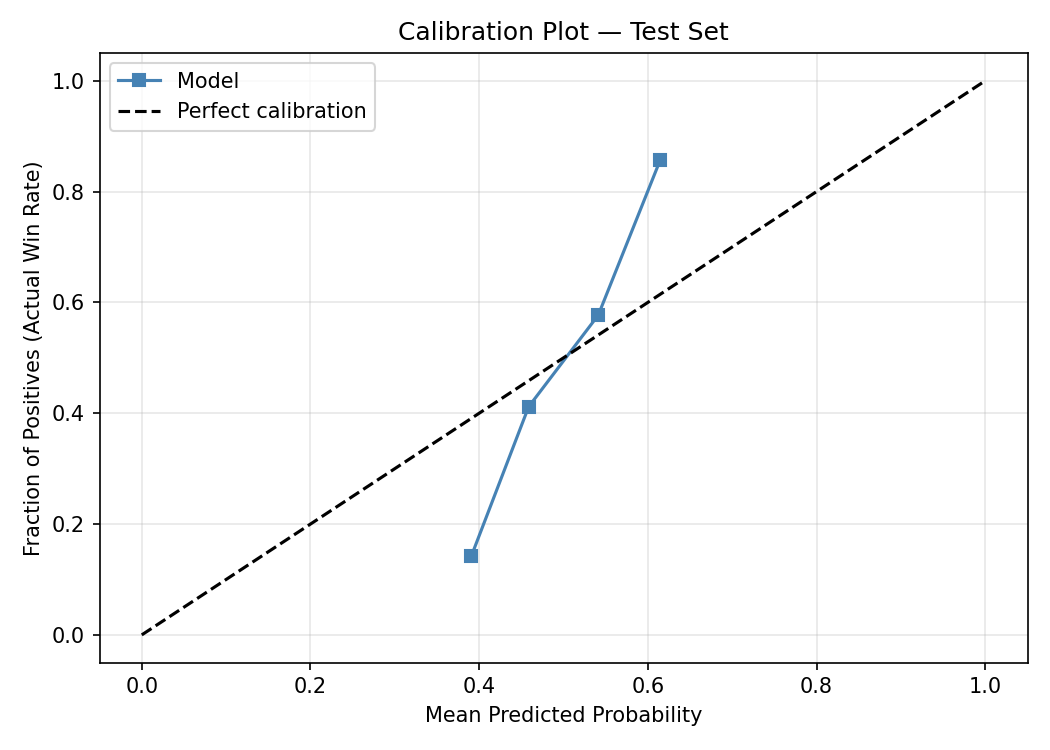
\includegraphics[width=\textwidth]{calibration_plot.png}
    \caption{Calibration: predicted vs observed.}
    \label{fig:cal}
  \end{subfigure}
  \hfill
  \begin{subfigure}[b]{0.47\textwidth}
    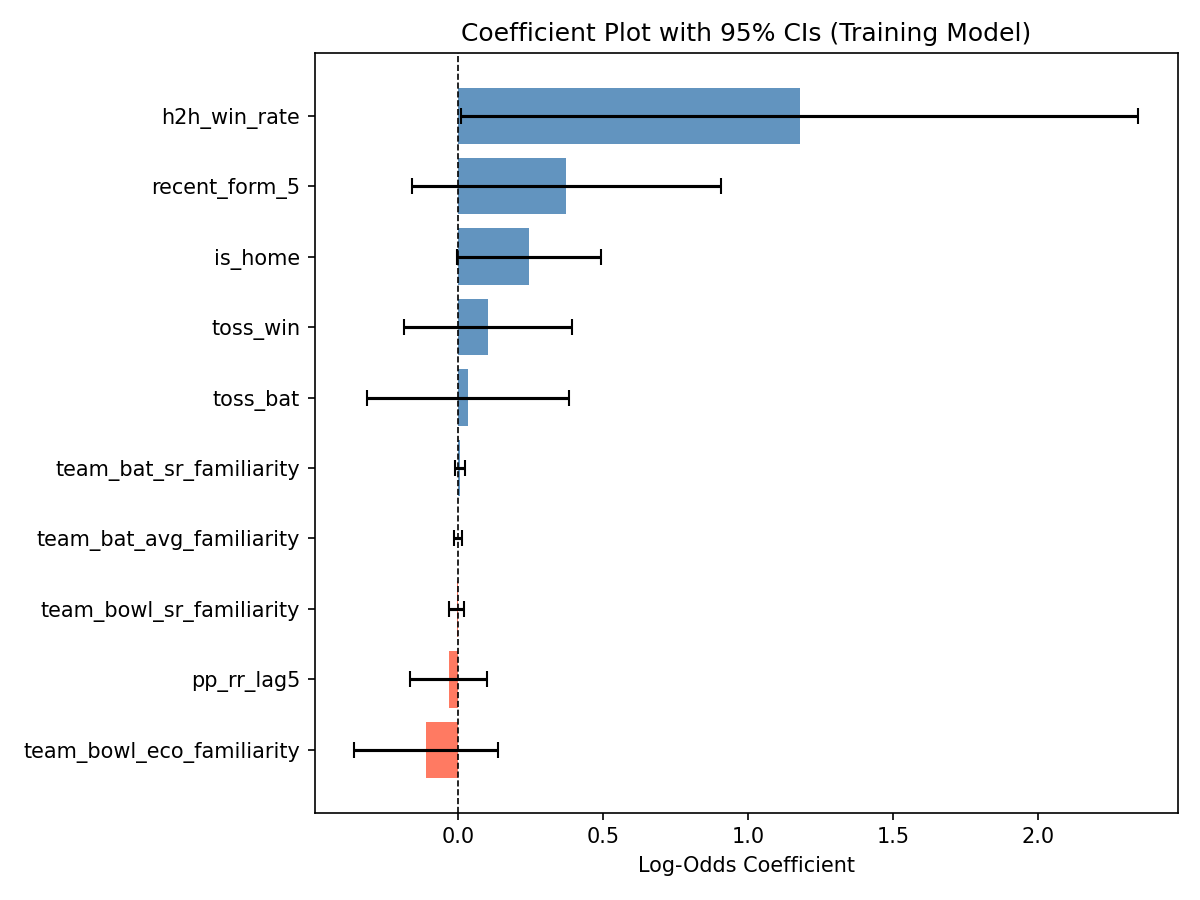
\includegraphics[width=\textwidth]{coefficient_plot.png}
    \caption{Coefficient plot with 95\% CIs.}
    \label{fig:coef}
  \end{subfigure}

  \vspace{0.5cm}

  \begin{subfigure}[b]{0.47\textwidth}
    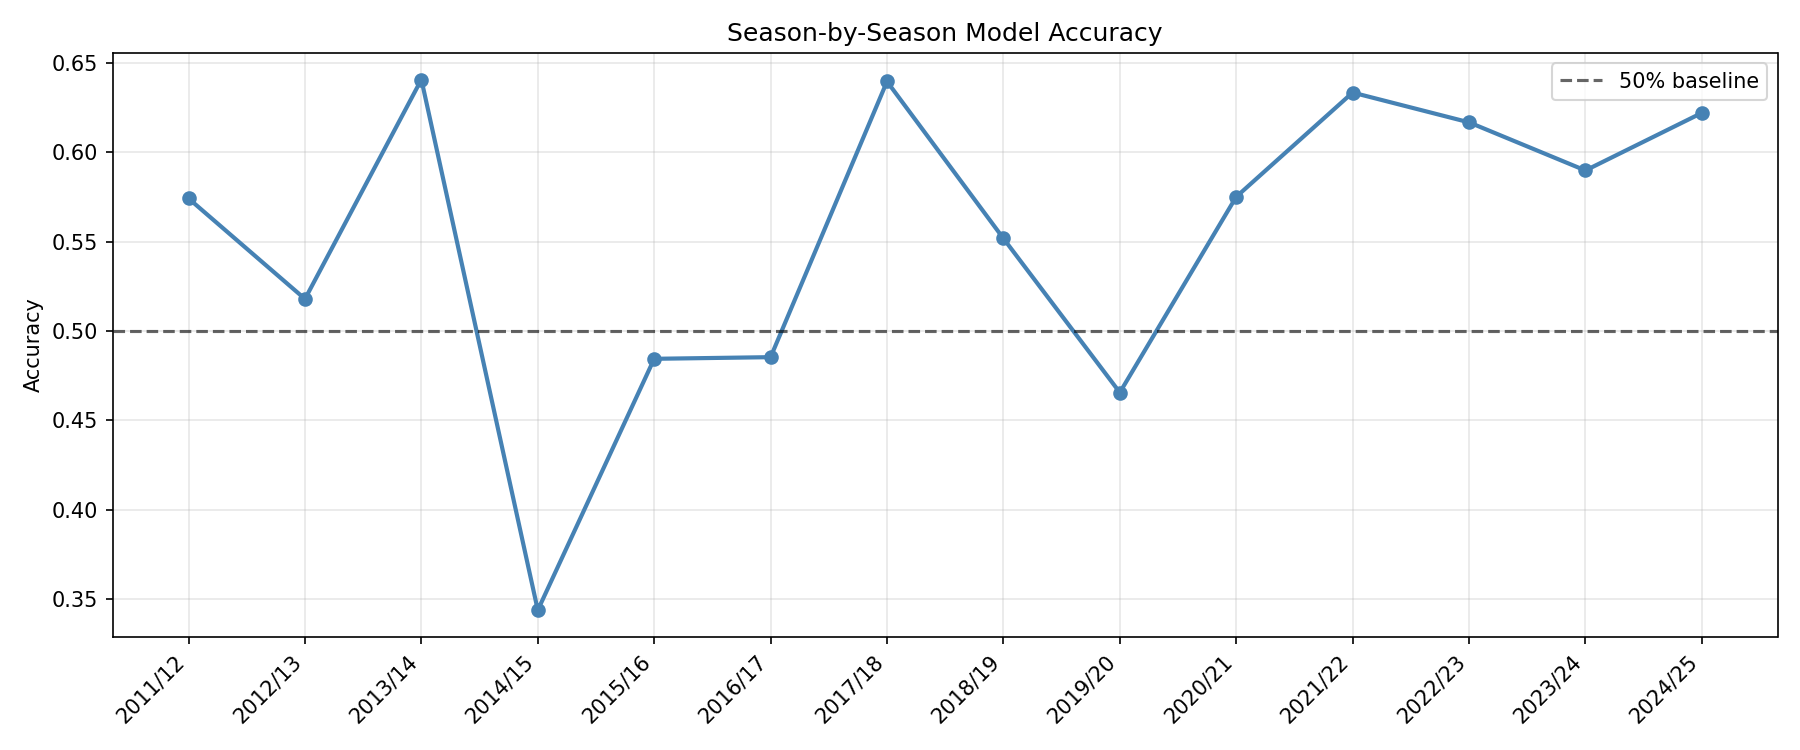
\includegraphics[width=\textwidth]{season_accuracy.png}
    \caption{Season-by-season M2 accuracy.}
    \label{fig:seasacc}
  \end{subfigure}
  \hfill
  \begin{subfigure}[b]{0.47\textwidth}
    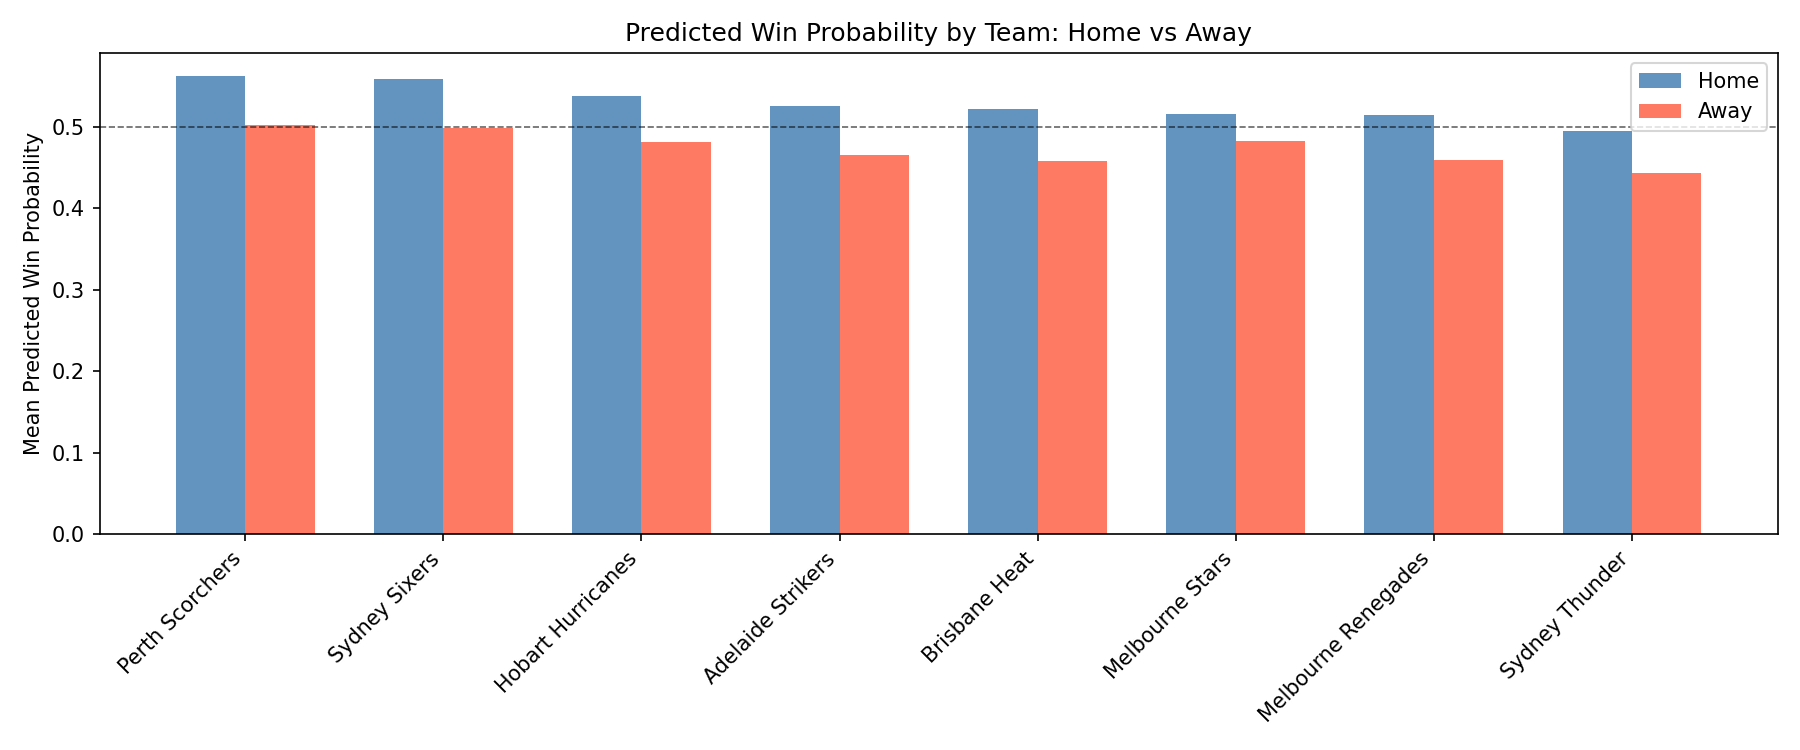
\includegraphics[width=\textwidth]{team_pred_prob.png}
    \caption{Predicted win probability by franchise.}
    \label{fig:teampred}
  \end{subfigure}

  \caption{M2 model diagnostics and performance figures.}
  \label{fig:m2diag}
\end{figure}

\subsubsection{M3: LASSO Interaction Model}

M3 tests whether predictors moderate each other. All 45 pairwise interactions are added to
the M2 predictors, then penalised via LASSO ($C = 0.05$). Surviving terms are re-fitted
without penalisation. The model is:
\[
  \log\frac{P(\text{win})}{1 - P(\text{win})} = \boldsymbol{\beta}^\top \mathbf{x}
    + \sum_{k \in \mathcal{S}} \gamma_k \,(x_{j_k} \cdot x_{l_k})
\]
where $\mathcal{S}$ is the set of interactions that survive LASSO shrinkage at $C = 0.05$.

Seven interactions survived (Table~\ref{tab:m3interactions}). None reached significance in
the unpenalised re-fit (all $p > 0.17$). AUC\,=\,0.663 ($\Delta$AUC\,=\,$-0.013$ vs M2);
AIC\,=\,1470.65, worse than M2. M2 is preferred.

\begin{table}[H]
\centering
\caption{M3: Interactions surviving LASSO ($C = 0.05$), re-fitted without penalisation.}
\label{tab:m3interactions}
\resizebox{\linewidth}{!}{%
\begin{tabular}{lcccc}
\toprule
\textbf{Interaction} & \textbf{LASSO coef.} & \textbf{Re-fit coef.} & \textbf{SE} & \textbf{$p$} \\
\midrule
\texttt{is\_home : toss\_win}                                    & $0.026$  & $0.086$  & $0.235$ & $0.715$ \\
\texttt{is\_home : recent\_form\_5}                              & $0.110$  & $0.493$  & $0.486$ & $0.310$ \\
\texttt{toss\_win : h2h\_win\_rate}                              & $0.016$  & $-0.042$ & $1.060$ & $0.969$ \\
\texttt{recent\_form\_5 : h2h\_win\_rate}                        & $0.032$  & $0.787$  & $2.228$ & $0.724$ \\
\texttt{h2h\_win\_rate : team\_bat\_sr\_familiarity}             & $0.000$  & $0.071$  & $0.062$ & $0.251$ \\
\texttt{h2h\_win\_rate : team\_bowl\_eco\_familiarity}           & $-0.080$ & $-0.014$ & $1.021$ & $0.989$ \\
\texttt{team\_bat\_sr\_familiarity : team\_bowl\_eco\_familiarity} & $-0.023$ & $-0.041$ & $0.037$ & $0.267$ \\
\bottomrule
\multicolumn{5}{l}{\small \texttt{is\_home} main effect: coef $= 0.072$, $p = 0.809$ (not significant in M3).}
\end{tabular}}
\end{table}

\subsubsection{M4: Bayesian GLMM}

M4 extends M2 by adding team- and match-level random intercepts, estimated via variational
Bayes (\texttt{statsmodels BinomialBayesMixedGLM}). The model is:
\[
  \text{logit}\!\left(P(\text{win}_{ij})\right)
    = \mathbf{x}_{ij}^\top \boldsymbol{\beta}
    + u_{\text{team}[i]}
    + u_{\text{match}[j]}
\]
\[
  u_{\text{team}} \sim \mathcal{N}(0,\,\sigma^2_{\text{team}}), \qquad
  u_{\text{match}} \sim \mathcal{N}(0,\,\sigma^2_{\text{match}})
\]

\begin{table}[H]
\centering
\caption{M4 posterior summary (variational Bayes). Random effects: team SD\,=\,0.294, match\_id SD\,=\,0.091.}
\label{tab:m4}
\small
\begin{tabular}{lcccc}
\toprule
\textbf{Predictor} & \textbf{Post. Mean} & \textbf{Post. SD} & \textbf{OR} & \textbf{$P(\beta > 0)$} \\
\midrule
Intercept                            & $-2.398$ & $0.058$ & $0.091$ & --- \\
\textbf{\texttt{is\_home}}           & $\mathbf{0.338}$ & $0.086$ & $\mathbf{1.402}$ & $\mathbf{100.00\%}$ \\
\texttt{toss\_win}                   & $0.224$  & $0.083$ & $1.251$ & $99.66\%$ \\
\texttt{toss\_bat}                   & $-0.106$ & $0.129$ & $0.900$ & $20.60\%$ \\
\texttt{recent\_form\_5}             & $0.260$  & $0.105$ & $1.297$ & $99.34\%$ \\
\texttt{h2h\_win\_rate}              & $0.501$  & $0.114$ & $1.650$ & $100.00\%$ \\
\texttt{pp\_rr\_lag5}                & $-0.006$ & $0.008$ & $0.994$ & $23.53\%$ \\
\texttt{team\_bat\_sr\_familiarity}  & $0.006$  & $0.001$ & $1.006$ & $100.00\%$ \\
\texttt{team\_bat\_avg\_familiarity} & $-0.003$ & $0.002$ & $0.998$ & $12.79\%$ \\
\texttt{team\_bowl\_eco\_familiarity}& $-0.142$ & $0.008$ & $0.867$ & $0.00\%$ \\
\texttt{team\_bowl\_sr\_familiarity} & $-0.005$ & $0.003$ & $0.995$ & $5.02\%$ \\
\bottomrule
\end{tabular}
\end{table}

The posterior probability that $\beta_{\text{is\_home}} > 0$ is 99.996\%. Fixed effects
track M2: \texttt{is\_home} OR\,=\,1.402 is unchanged after accounting for team and
match-level clustering. Random effect SDs: team\,=\,0.294, \texttt{match\_id}\,=\,0.091.

Team-level posterior probability of a positive home effect: Perth Scorchers (98.2\%),
Adelaide Strikers (94.5\%), Hobart Hurricanes (94.5\%), Melbourne Stars (85.2\%), Sydney
Sixers (84.8\%), Sydney Thunder (84.7\%), Melbourne Renegades (51.9\%), Brisbane Heat
(24.7\%). These values represent the posterior evidence for a positive team-level home
coefficient, not literal predicted home win probabilities.

\subsubsection{M5: \texttt{lme4 glmer}, Gold-Standard Specification}

M5 uses the same mixed-effects specification as M4 but is estimated via the Laplace
approximation in R's \texttt{lme4} package (called through \texttt{rpy2}), which is the
standard reference implementation for GLMMs. The model is identical in structure to M4:
\[
  \text{logit}\!\left(P(\text{win}_{ij})\right)
    = \mathbf{x}_{ij}^\top \boldsymbol{\beta}
    + u_{\text{team}[i]}
    + u_{\text{match}[j]}
\]
\[
  u_{\text{team}} \sim \mathcal{N}(0,\,\hat\sigma^2_{\text{team}}), \qquad
  u_{\text{match}} \sim \mathcal{N}(0,\,\hat\sigma^2_{\text{match}})
\]

\begin{table}[H]
\centering
\caption{M5 fixed effects (\texttt{lme4 glmer}; \texttt{match\_id} SD\,=\,0, team SD\,=\,0.217).}
\label{tab:m5}
\small
\begin{tabular}{lcccc}
\toprule
\textbf{Predictor} & \textbf{Coef.} & \textbf{SE} & \textbf{$p$} & \textbf{OR} \\
\midrule
Intercept                            & $-3.099$ & $1.115$ & $0.005$ & --- \\
\textbf{\texttt{is\_home}}           & $\mathbf{0.339}$ & $0.119$ & $\mathbf{0.004}$ & $\mathbf{1.404}$ \\
\texttt{toss\_win}                   & $0.223$  & $0.137$ & $0.104$ & $1.249$ \\
\texttt{toss\_bat}                   & $-0.096$ & $0.170$ & $0.572$ & $0.908$ \\
\texttt{recent\_form\_5}             & $0.304$  & $0.269$ & $0.258$ & $1.356$ \\
\texttt{h2h\_win\_rate}              & $0.739$  & $0.628$ & $0.239$ & $2.094$ \\
\texttt{pp\_rr\_lag5}                & $0.005$  & $0.066$ & $0.945$ & $1.005$ \\
\texttt{team\_bat\_sr\_familiarity}  & $0.008$  & $0.008$ & $0.355$ & $1.008$ \\
\texttt{team\_bat\_avg\_familiarity} & $-0.003$ & $0.007$ & $0.625$ & $0.997$ \\
\texttt{team\_bowl\_eco\_familiarity}& $-0.169$ & $0.128$ & $0.186$ & $0.845$ \\
\texttt{team\_bowl\_sr\_familiarity} & $-0.006$ & $0.013$ & $0.664$ & $0.994$ \\
\bottomrule
\end{tabular}
\end{table}

The \texttt{match\_id} random effect goes singular: once \texttt{is\_home} is in the model,
no residual within-match correlation remains. Team variance is non-zero (SD\,=\,0.217),
pointing to small but real franchise-level differences. \texttt{is\_home} is significant at
$p = 0.004$, consistent with M2.

\begin{table}[H]
\centering
\caption{Model comparison summary.}
\label{tab:comparison}
\begin{tabular}{llccc}
\toprule
\textbf{Model} & \textbf{Description} & \textbf{AUC} & \textbf{Accuracy} & \textbf{AIC} \\
\midrule
M1 & Baseline logit         & 0.613 & 61.3\% & 1453.83 \\
M2 & Full logit             & 0.676 & 60.6\% & 1460.98 \\
M3 & LASSO interactions     & 0.663 & 61.9\% & 1470.65 \\
M4 & Bayesian GLMM          & $\approx$0.676 & $\approx$61\% & --- \\
M5 & \texttt{lme4 glmer}    & $\approx$0.676 & $\approx$61\% & 1671.9$^\dagger$ \\
\bottomrule
\multicolumn{5}{l}{\small $^\dagger$M5 AIC includes random effect parameters; not comparable to M1 to M3.}
\end{tabular}
\end{table}

Although M1 has the lower AIC because it is more parsimonious, M2 is retained as the
primary inferential model because it tests whether home advantage survives after controlling
for form, head-to-head history, toss outcome, and familiarity metrics, and it improves
holdout discrimination.

\subsection{Extended Analysis: Robustness and Match Context}
\label{sec:extended}

A parallel analysis (\texttt{BBL\_Extended\_Analysis.ipynb}) uses one row per match to test
home advantage from a different angle and examine match-phase effects. The results
corroborate M1 to M5; they do not replace them.

\subsubsection{Toss and First-Innings Effects}

Three two-sided binomial tests ($H_0: \pi = 0.5$, $\alpha = 0.05$):
\begin{enumerate}
  \item Toss winner wins match: $\hat{p} = 0.523$, $p = 0.272$, \textbf{not significant}
  \item Batting-first team wins: $\hat{q} = 0.482$, $p = 0.393$, \textbf{not significant}
  \item Toss winner who bats first wins: $\hat{r} = 0.506$, $p = 0.899$, \textbf{not significant}
\end{enumerate}

Captains chose to field 59\% of the time (357/604), consistent with the T20 preference for
chasing. It did not translate into higher win rates.

\begin{figure}[H]
  \centering
  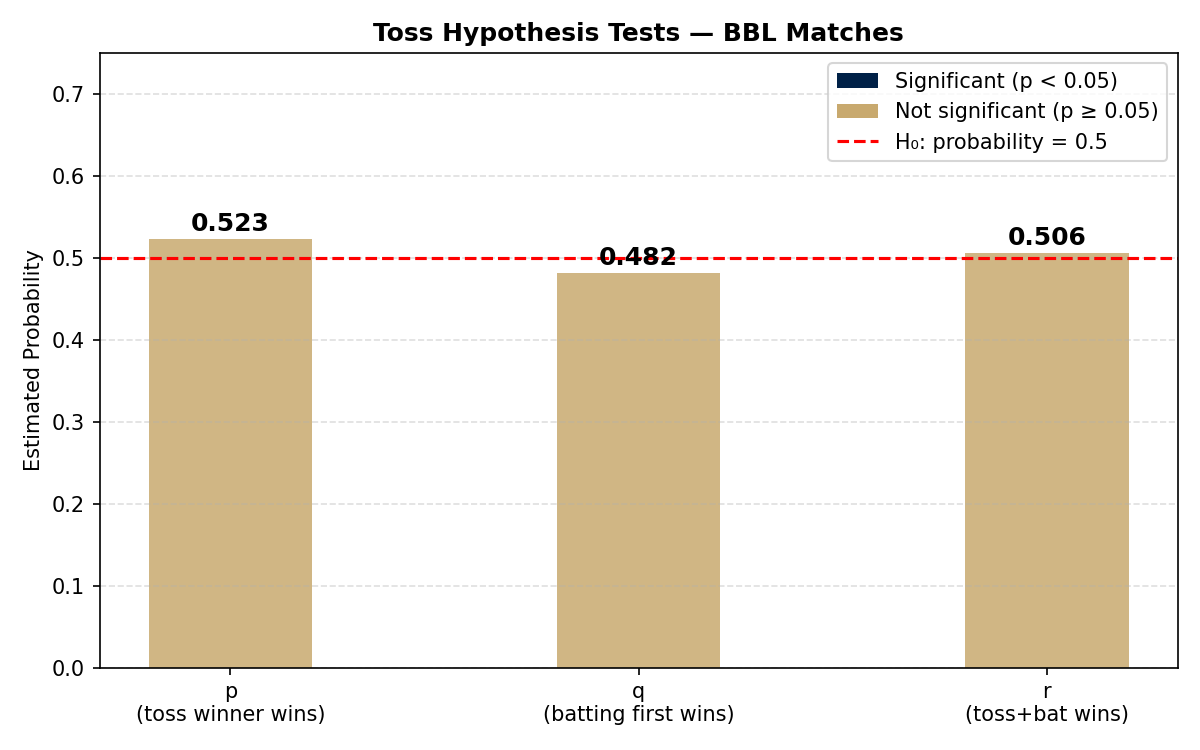
\includegraphics[width=0.75\textwidth]{toss_hypothesis_tests.png}
  \caption{Binomial hypothesis test results for toss-related outcomes.}
  \label{fig:toss}
\end{figure}

\subsubsection{Innings-Phase Effects}

Logistic regression of batting-first win on first-innings runs: AUC\,=\,0.769,
Pseudo~$R^2 = 0.172$, accuracy\,=\,70.2\% ($p < 0.001$). The 50\% break-even is
\textbf{162 runs}, matching the observed mean (161.4, SD\,=\,28.3). Above 175 runs, teams
win roughly 65\% of matches. After controlling for score, \texttt{is\_home} is non-significant
($\hat{\beta} = 0.209$, $p = 0.257$, OR\,=\,1.23): home advantage does not operate within
the scoring phase.

\begin{figure}[H]
  \centering
  \begin{subfigure}[b]{0.47\textwidth}
    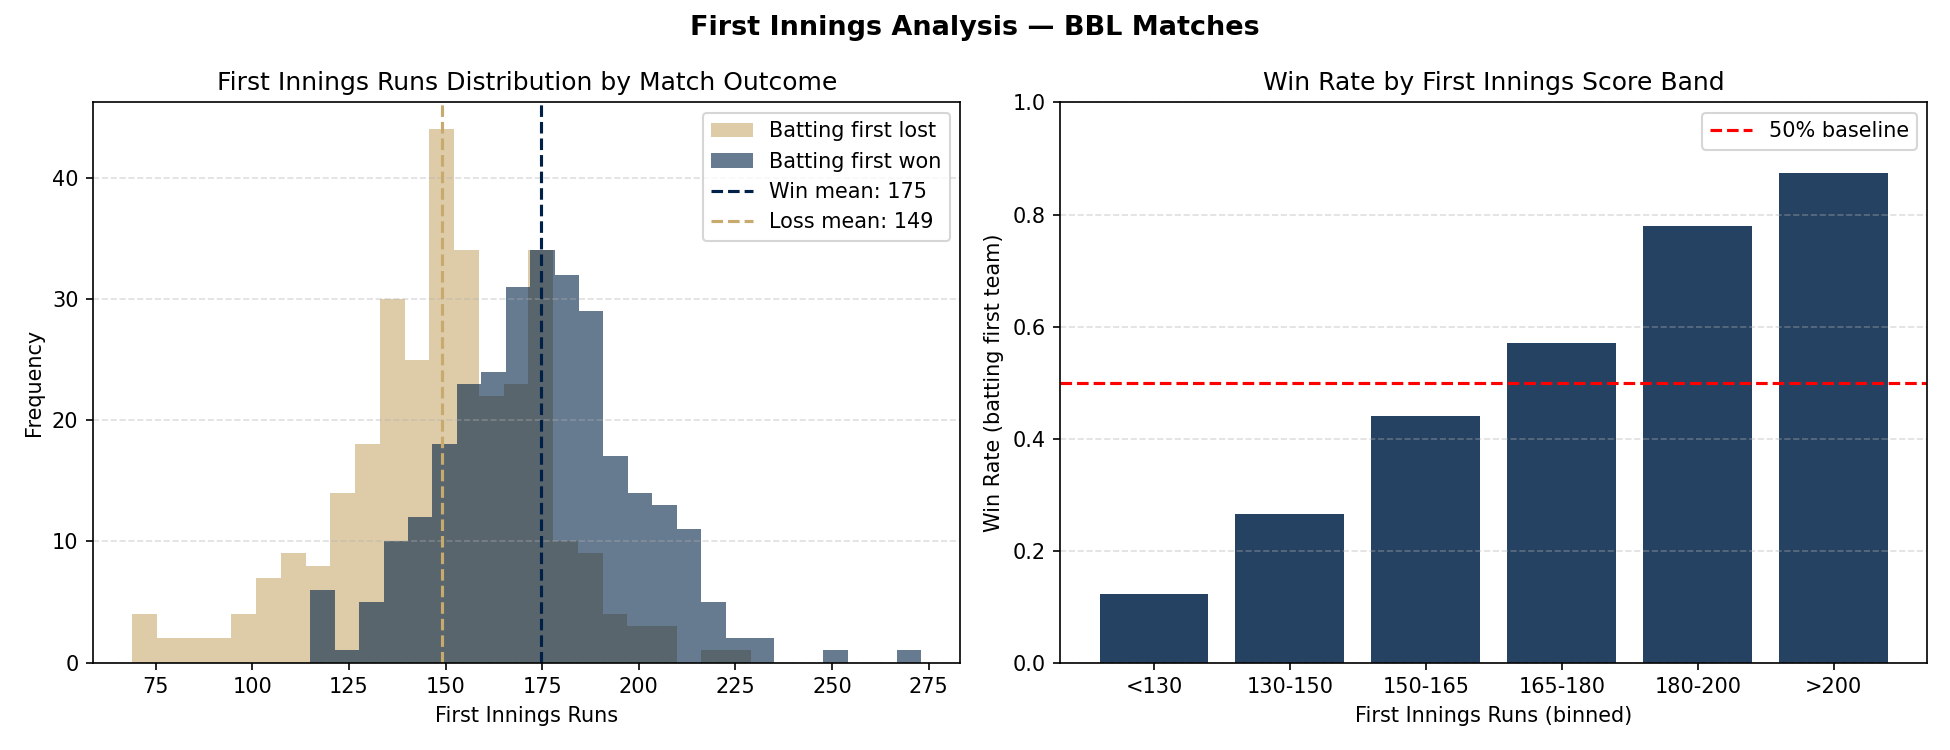
\includegraphics[width=\textwidth]{first_innings_distribution.png}
    \caption{First-innings score distribution by outcome.}
  \end{subfigure}
  \hfill
  \begin{subfigure}[b]{0.47\textwidth}
    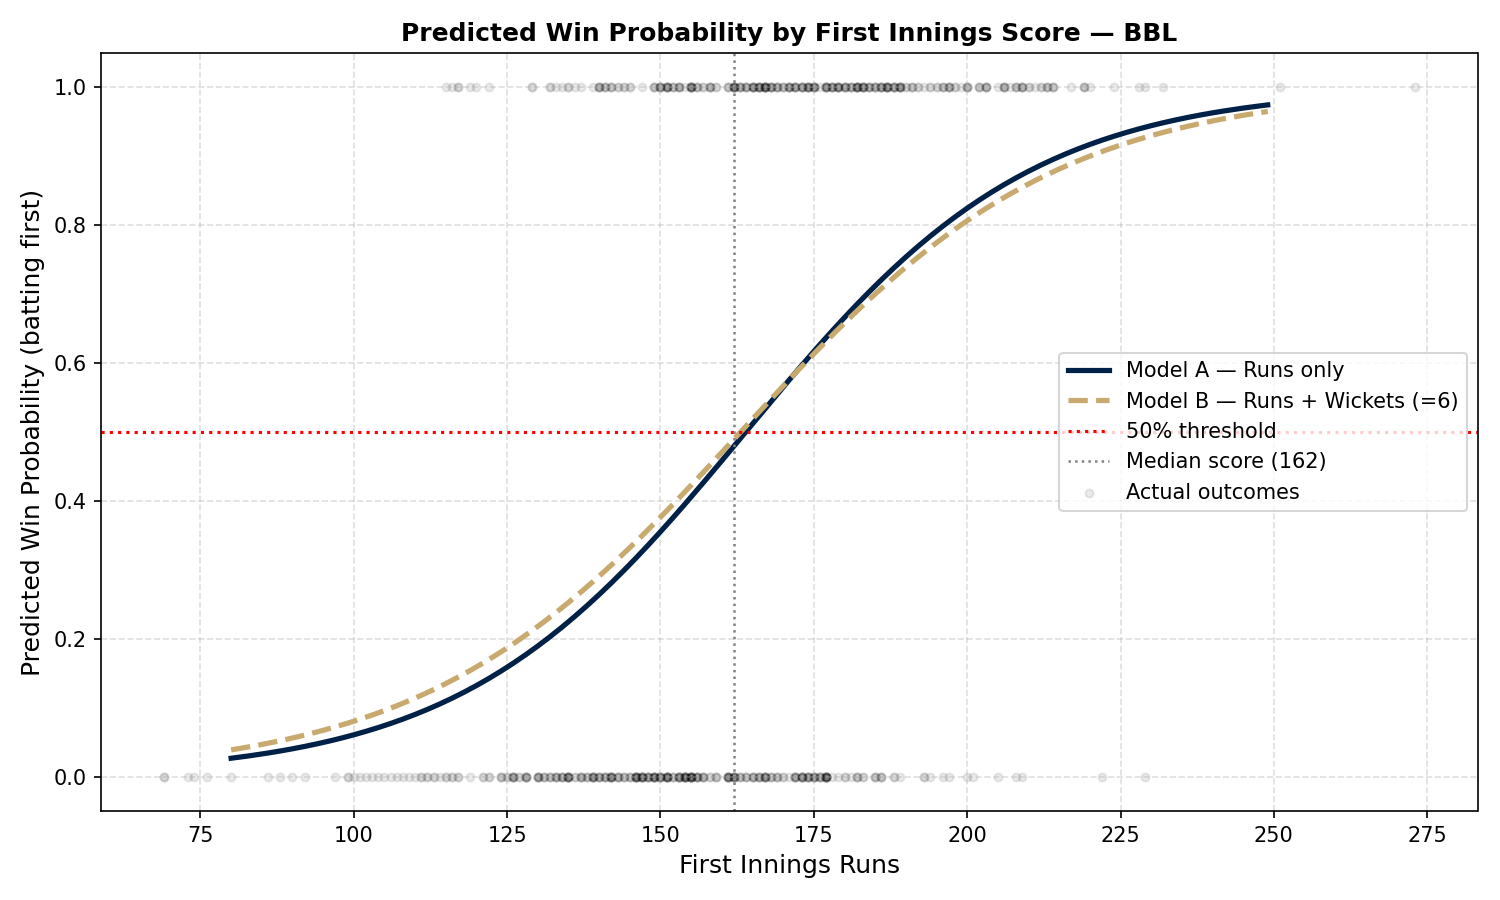
\includegraphics[width=\textwidth]{first_innings_prediction_curve.png}
    \caption{Win probability S-curves (break-even $\approx$ 162 runs).}
  \end{subfigure}
  \caption{First innings analysis.}
  \label{fig:firstinn}
\end{figure}

\begin{figure}[H]
  \centering
  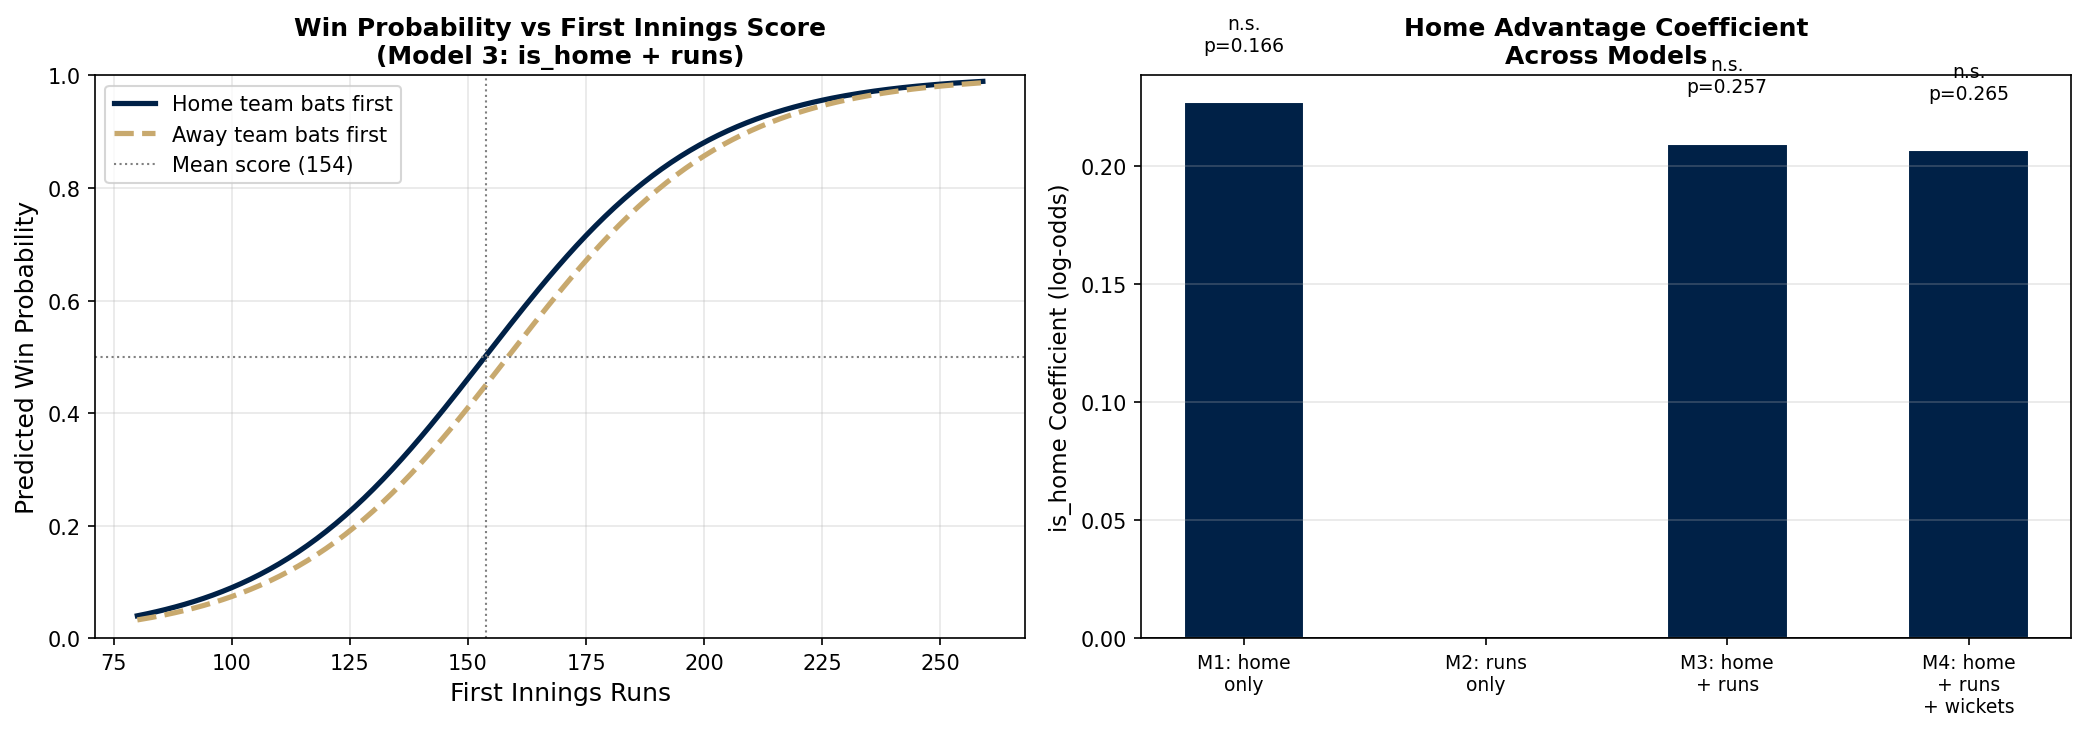
\includegraphics[width=0.78\textwidth]{section3_combined_model.png}
  \caption{Win probability curves and \texttt{is\_home} coefficients across extended analysis
  models (EA-1 to EA-4).}
  \label{fig:ea}
\end{figure}

\subsubsection{Season Variation in Home Advantage}

The home advantage gap ran from $-0.235$ (2016/17) to $+0.411$ (2024/25). A positive trend
of $+0.025$ per season suggests the gap has grown over time, consistent with franchise
identities, supporter cultures, and ground familiarity maturing as the league aged. Per-season
samples of $\approx$43 matches are too small to be confident in the slope year-by-year, but
the pooled trend across 14 seasons is consistent.

\begin{figure}[H]
  \centering
  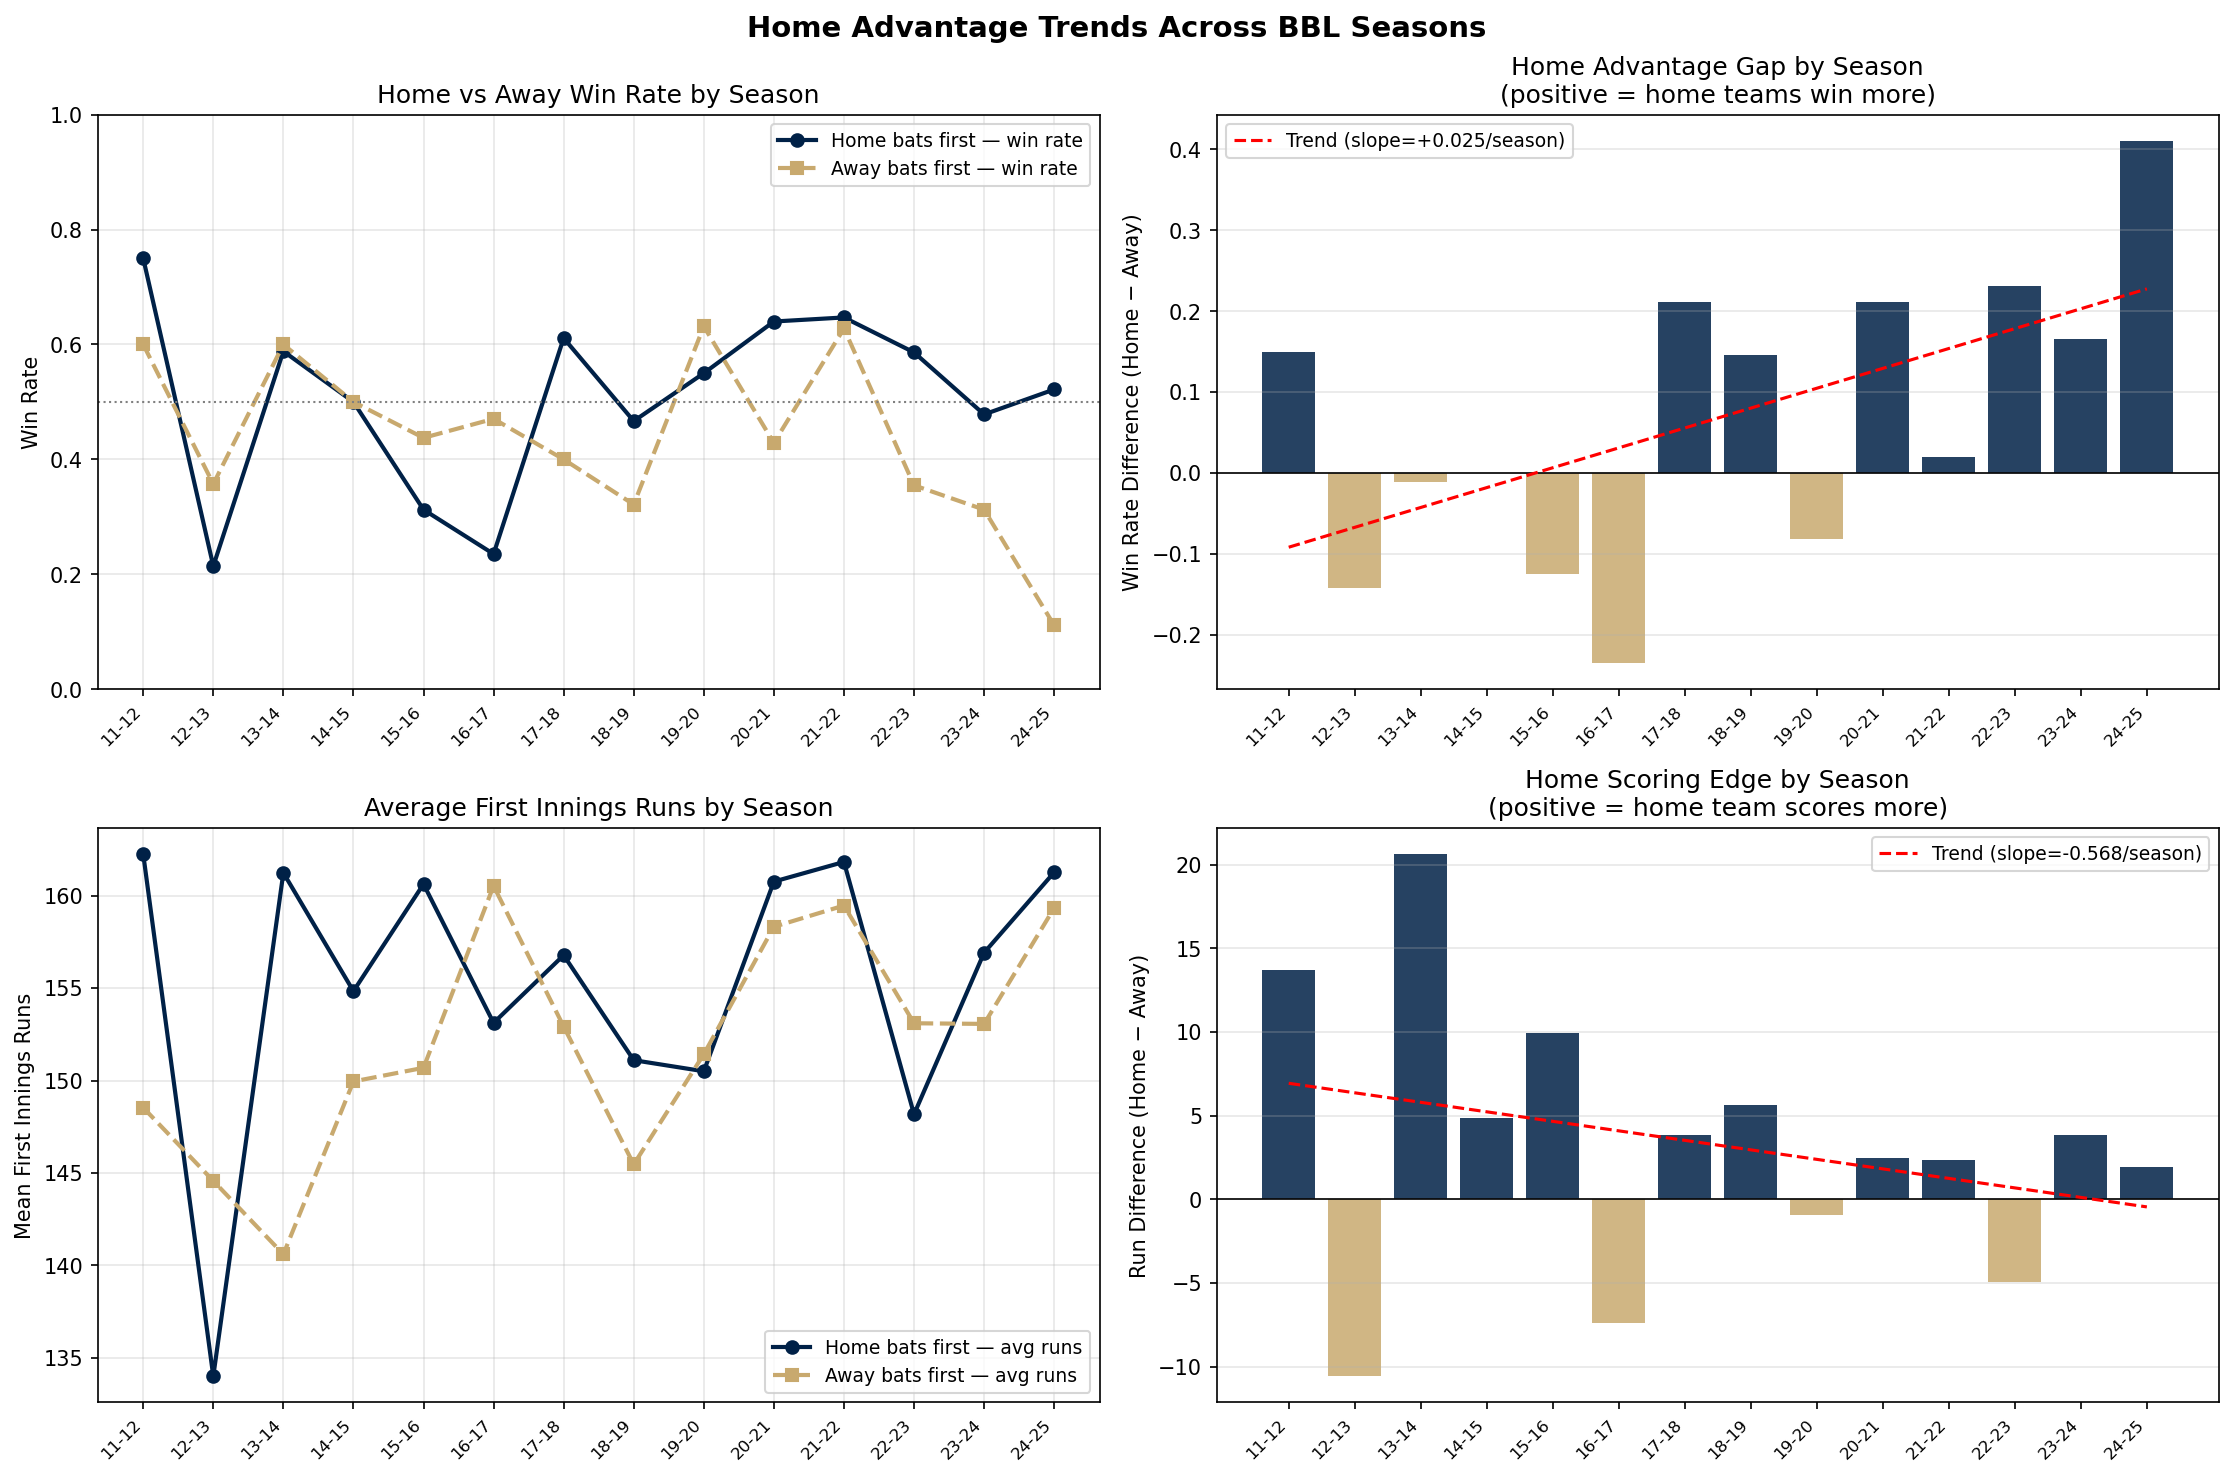
\includegraphics[width=0.88\textwidth]{section4_season_trends.png}
  \caption{Season trends in home/away win rates, home advantage gap, and first-innings scores.}
  \label{fig:seasons}
\end{figure}

\subsubsection{Venue-Level Differences}

Adelaide Strikers ($+0.131$ gap, $+15.3$-run scoring edge) and Perth Scorchers ($+0.124$
gap, $+5.9$-run scoring edge) have the largest home advantages through different mechanisms.
Brisbane Heat is the only franchise with a negative gap ($-0.051$).

\begin{figure}[H]
  \centering
  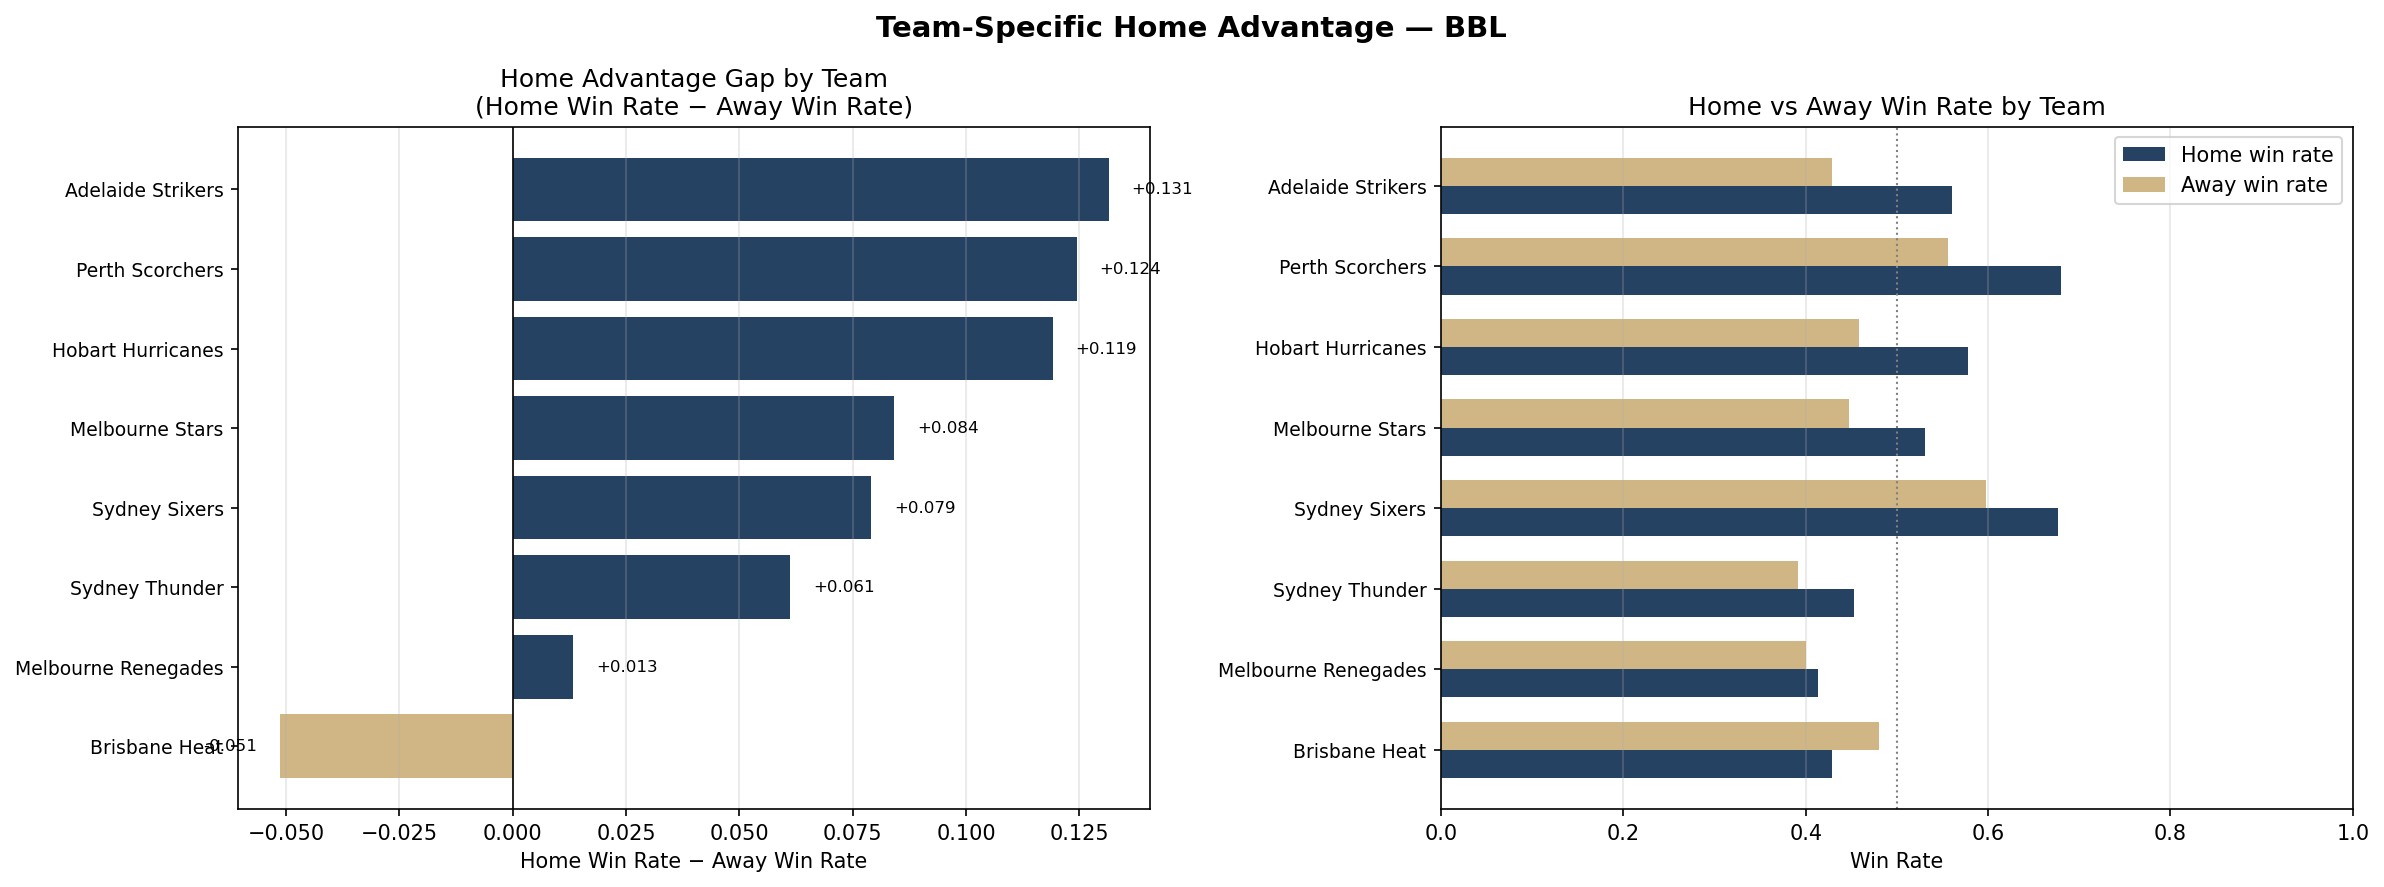
\includegraphics[width=0.88\textwidth]{section5_team_home_advantage.png}
  \caption{Team-specific home advantage gap and win rates by franchise.}
  \label{fig:teamha}
\end{figure}

\subsubsection{COVID and Neutral-Venue Robustness}

BBL seasons 10/11 (2020 to 2022) involved hub-based scheduling at non-primary venues, raising
questions about whether home-team classifications in those seasons are reliable. The robustness
checks in Section~\ref{sec:robust} address this directly: excluding COVID seasons leaves the
home advantage finding unchanged (OR\,=\,1.31, $p = 0.040$), and restricting to primary
venues strengthens it (OR\,=\,1.54, $p = 0.001$). The COVID period produced a larger home advantage estimate, which argues against crowd noise
as the primary mechanism.

\subsubsection{DRS Umpiring Bias}
\label{sec:drs}

156 DRS reviews across seasons 12 to 14: home teams overturned 31.6\% (25/79), away teams
28.6\% (22/77). $\chi^2 = 0.059$, $p = 0.807$. No umpiring bias is detectable, though
$n = 156$ is too small to rule it out. Six to eight seasons of DRS data would give the test
adequate power.

\begin{figure}[H]
  \centering
  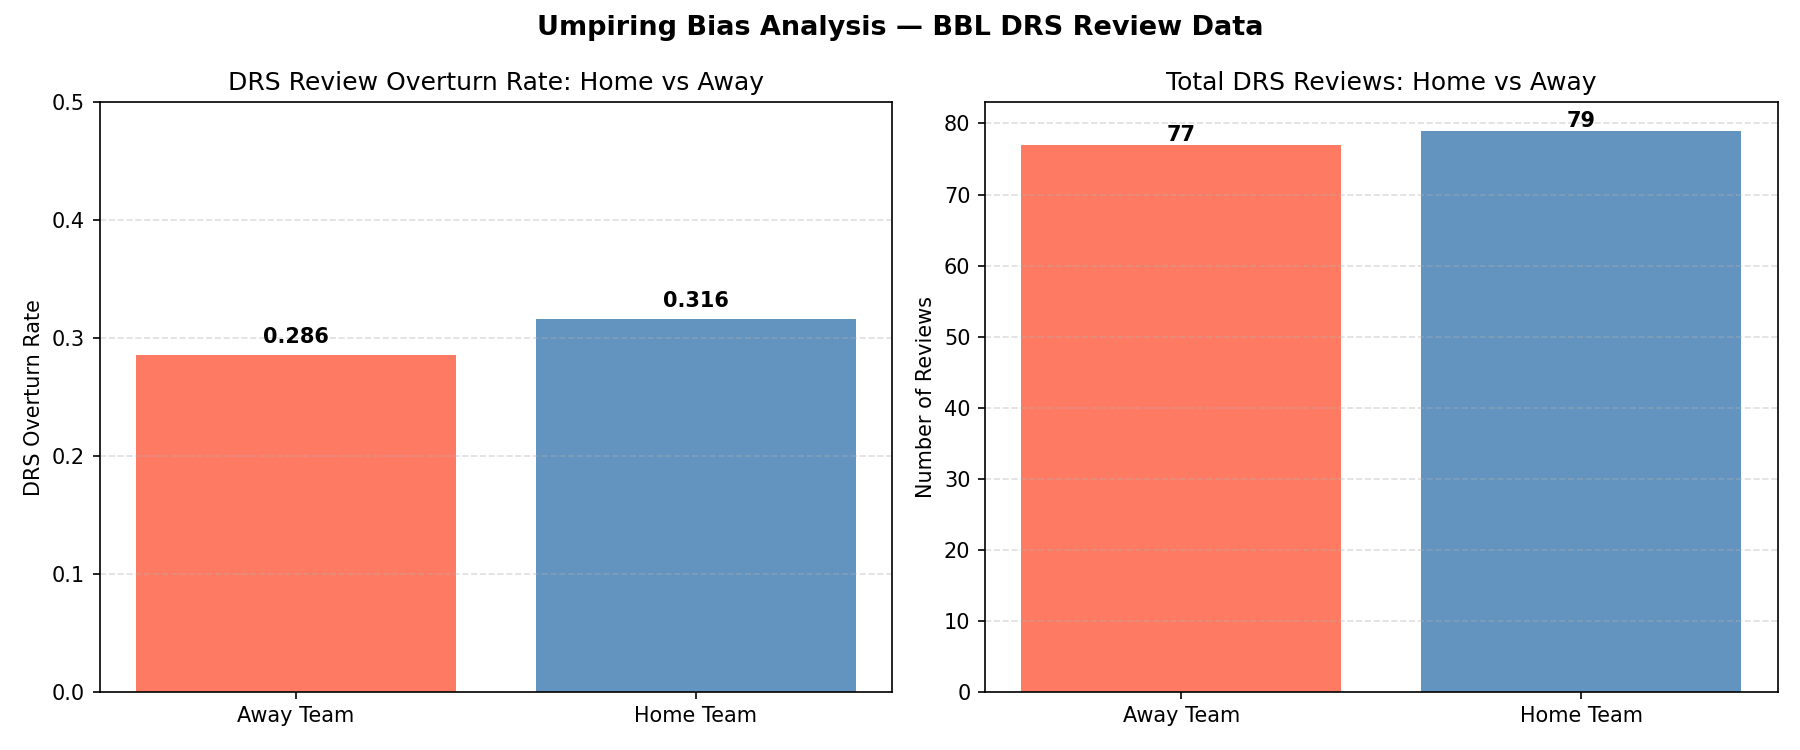
\includegraphics[width=0.70\textwidth]{umpiring_bias.png}
  \caption{DRS review overturn rates: home (31.6\%) vs away (28.6\%), not significant.}
  \label{fig:drs}
\end{figure}

\subsubsection{Mixed-Effects in the Extended Analysis}

Adding \texttt{(1|home\_team)} or \texttt{(1|venue)} random intercepts to the first-innings
model yields log-SDs near $-8$ to $-15$, effectively zero. \texttt{is\_home} stays
non-significant across all specifications.

\begin{figure}[H]
  \centering
  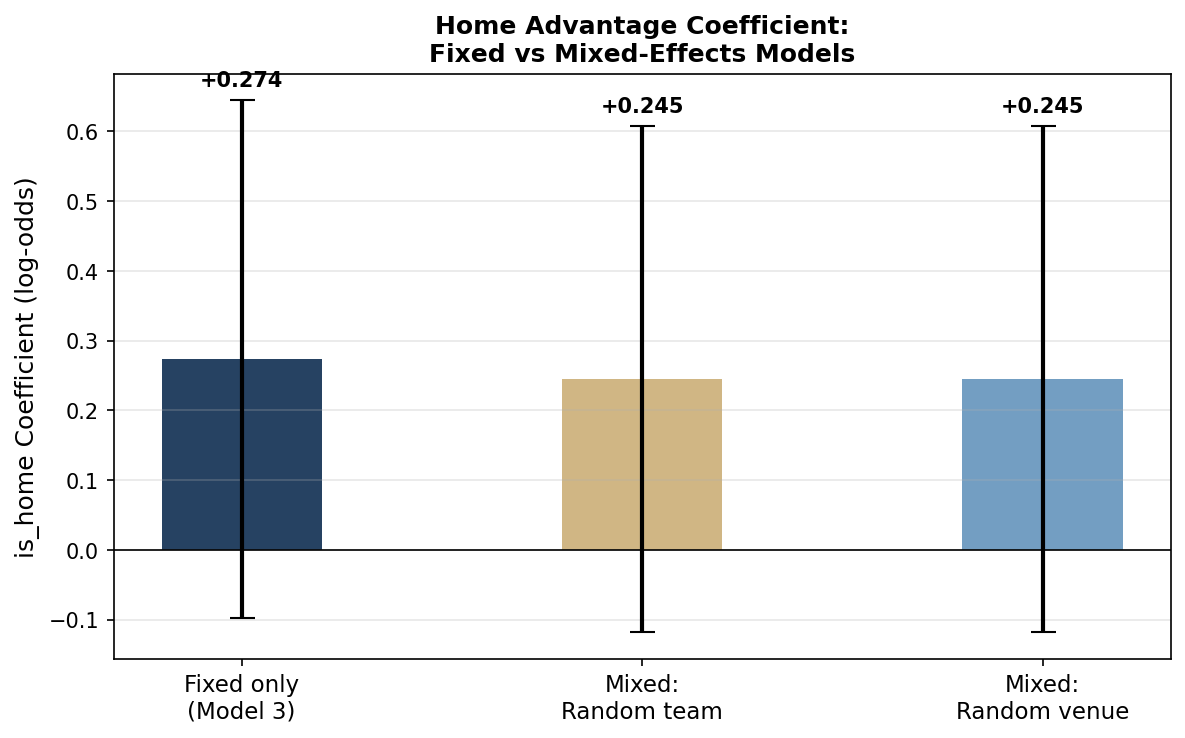
\includegraphics[width=0.78\textwidth]{section7_mixed_effects.png}
  \caption{\texttt{is\_home} coefficient across fixed-effects and mixed-effects model
  specifications.}
  \label{fig:me}
\end{figure}

\subsubsection{Home Bowling Defence}

When the home team bowled second, their defence success rate was 51.3\% versus 43.3\% for
away bowling teams. Controlling for the first-innings total removes the gap:
\texttt{is\_home\_bowling} OR\,=\,1.312, $p = 0.152$. Second-innings economy rates were
also indistinguishable ($p = 0.754$). Home advantage is not a bowling defence phenomenon.

\begin{figure}[H]
  \centering
  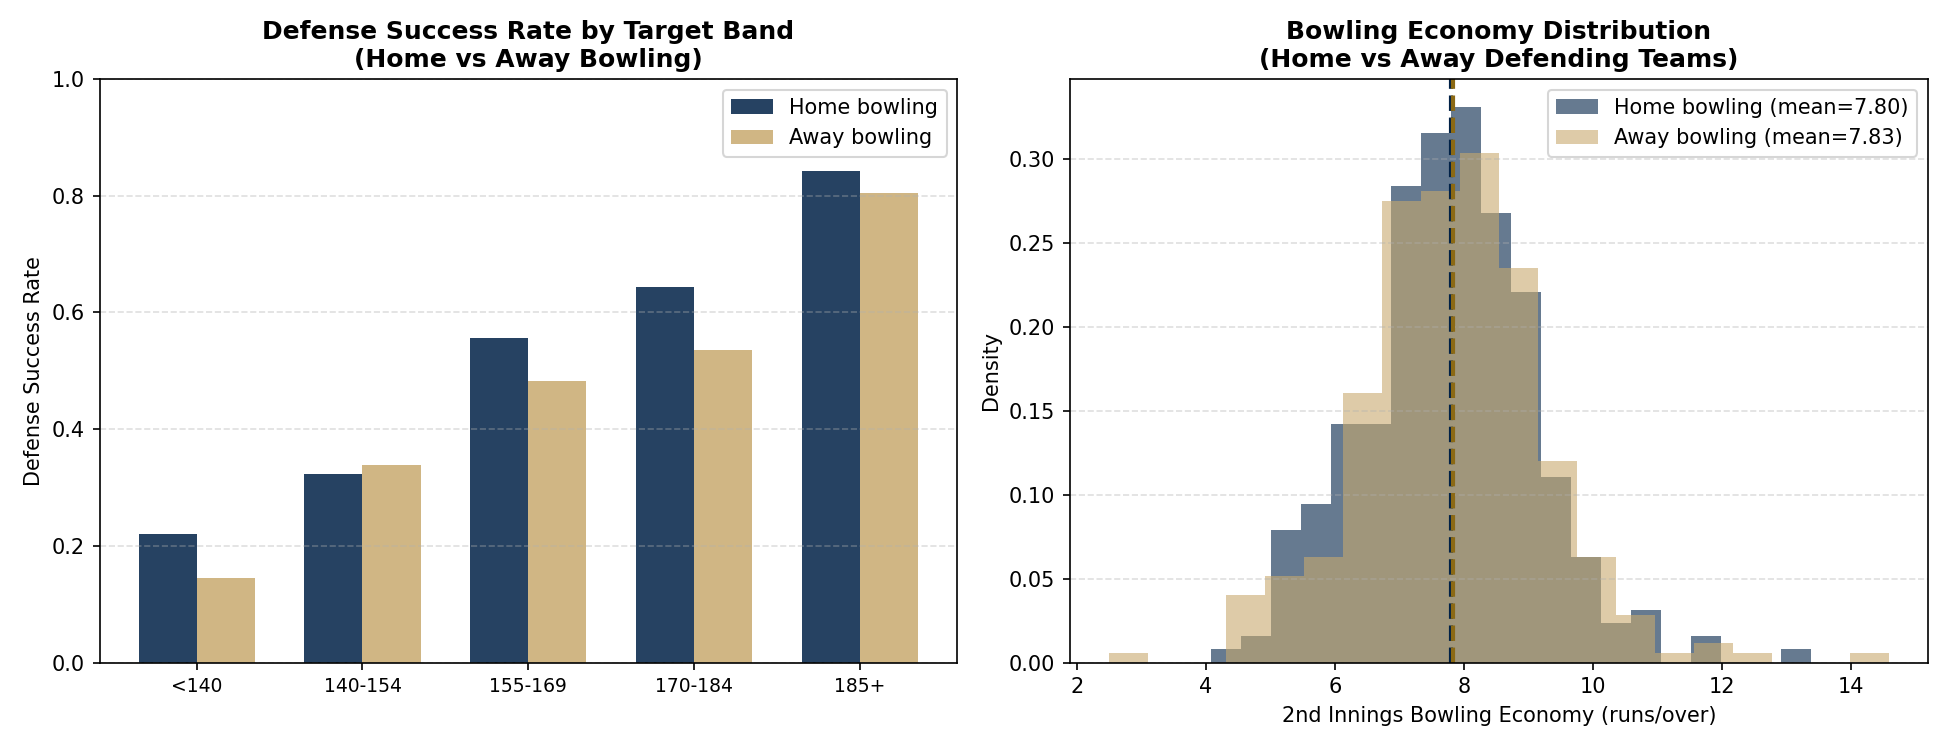
\includegraphics[width=0.82\textwidth]{home_bowling_defense.png}
  \caption{Defence success rate by target band and bowling economy distribution, home vs away.}
  \label{fig:bowl}
\end{figure}

\subsubsection{First-Six-Over Phase}

Home teams lost 1.569 wickets per innings in the first-six-over phase on average; away teams
1.571 ($p = 0.979$). Run rates over the same phase: 7.389 vs 7.317 runs/over ($p = 0.535$).
Away batters show no signs of struggling in unfamiliar conditions during the first six overs.
Home advantage does not operate through first-six-over suppression.

\begin{figure}[H]
  \centering
  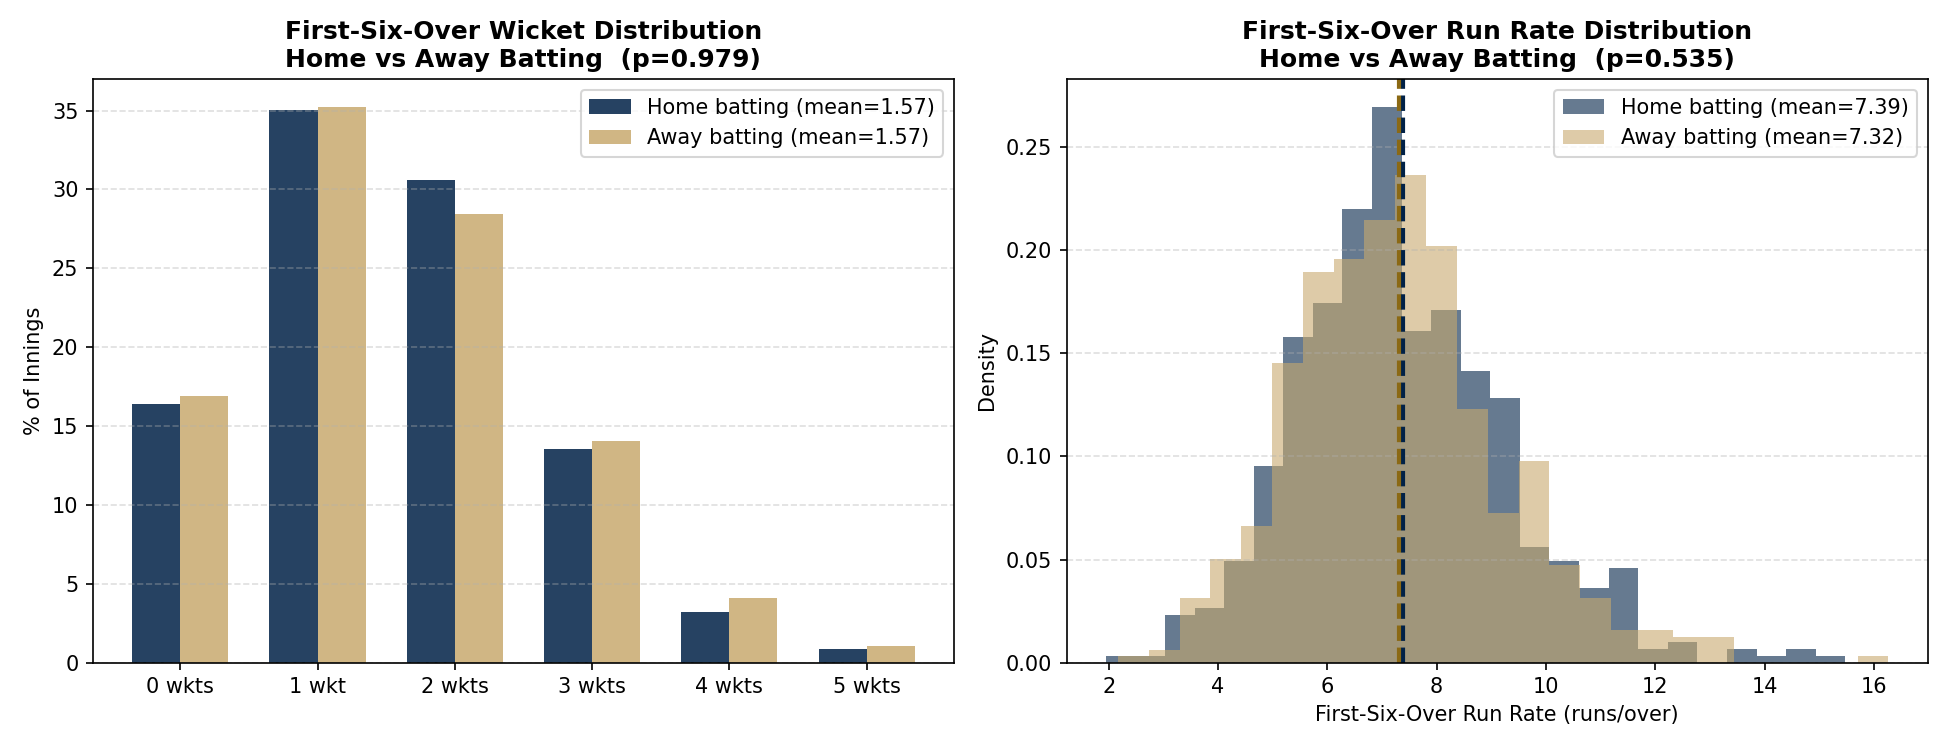
\includegraphics[width=0.82\textwidth]{powerplay_home_vs_away.png}
  \caption{First-six-over wicket distribution and run rate by home vs away batting.}
  \label{fig:pp}
\end{figure}

\subsubsection{Summary of Extended Findings}
\label{sec:extsummary}

Across all extended analyses, the same pattern holds: home advantage is detectable at the
match level but not within specific innings phases. Toss confers no reliable advantage.
First-innings score is the strongest in-match predictor once the game is underway. DRS data
show no umpiring bias, though the sample is underpowered. Season trends suggest the gap has grown over 14 seasons, led by franchises with established
venue cultures (Adelaide Strikers, Hobart Hurricanes). None of these analyses contradict
M1 to M5; they sharpen where home advantage operates and where it does not.

\subsubsection{Robustness Checks}
\label{sec:robust}

\textbf{Check 1: Primary venues only.} Restricting to established primary home grounds
(494 of 604 matches) strengthens the result: M1 OR\,=\,1.526 ($p = 0.001$); M2
OR\,=\,1.543 ($p = 0.001$).

\textbf{Check 2: COVID-era sensitivity.} Excluding BBL seasons 10/11 (484 matches),
\texttt{is\_home} remains significant in both models (M1: OR\,=\,1.314, $p = 0.034$; M2:
OR\,=\,1.313, $p = 0.040$). COVID-era subset: M2 OR\,=\,1.717, $p = 0.069$ ($n = 120$).

\textbf{Check 3: Season-by-season stability.} M1 estimated separately for each of 14
seasons. OR positive in 7 of 14; 3 seasons reach individual significance (2020/21, 2022/23,
2024/25). Pooled estimate is significant because later, larger seasons dominate.

\begin{table}[H]
\centering
\caption{\texttt{is\_home} robustness across subsets and models.}
\label{tab:robust}
\small
\begin{tabular}{llcccc}
\toprule
\textbf{Subset} & \textbf{Model} & \textbf{N} & \textbf{OR} & \textbf{95\% CI} & \textbf{$p$} \\
\midrule
Full dataset                     & M1 & 604 & 1.359 & (1.083, 1.705) & 0.008** \\
Full dataset                     & M2 & 604 & 1.391 & (1.103, 1.755) & 0.005** \\
Non-COVID (excl.\ BBL10/11)     & M1 & 484 & 1.314 & (1.021, 1.692) & 0.034** \\
Non-COVID (excl.\ BBL10/11)     & M2 & 484 & 1.313 & (1.013, 1.700) & 0.040** \\
COVID-only (BBL10/11)           & M1 & 120 & 1.588 & (0.939, 2.687) & 0.085$^\dagger$ \\
COVID-only (BBL10/11)           & M2 & 120 & 1.717 & (0.958, 3.076) & 0.069$^\dagger$ \\
Primary venues only              & M1 & 494 & 1.526 & (1.187, 1.961) & 0.001*** \\
Primary venues only              & M2 & 494 & 1.543 & (1.193, 1.995) & 0.001*** \\
\bottomrule
\multicolumn{6}{l}{\small $^\dagger$ $p < 0.10$; ** $p < 0.05$; *** $p < 0.01$}
\end{tabular}
\end{table}

\begin{figure}[H]
  \centering
  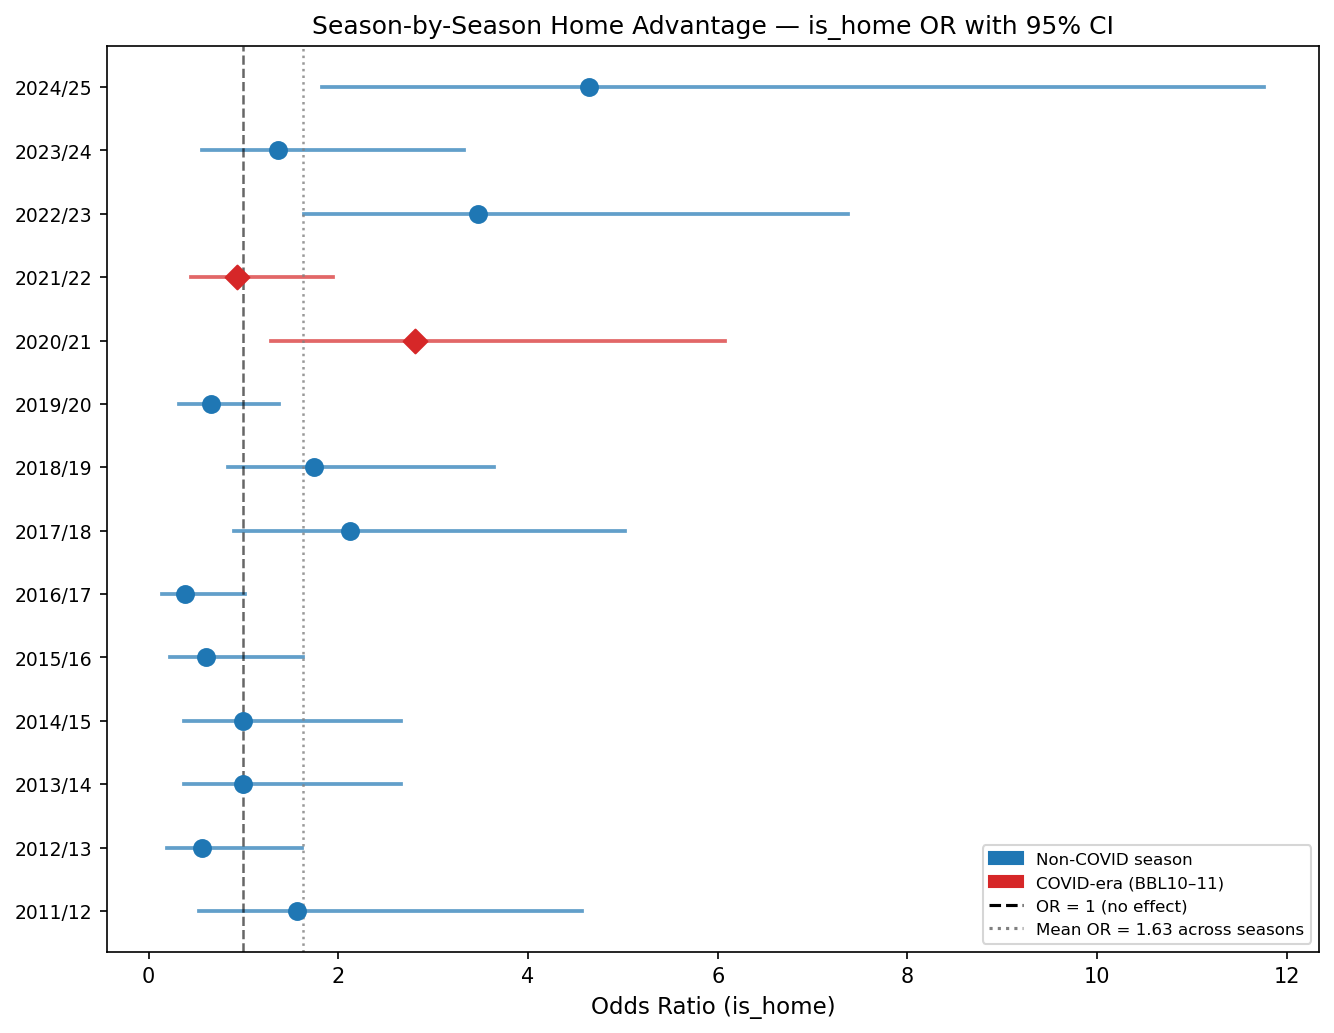
\includegraphics[width=0.88\textwidth]{robustness_season_forest.png}
  \caption{Season-by-season \texttt{is\_home} OR with 95\% CI. COVID-era seasons
  (BBL10/11) marked in red.}
  \label{fig:forest}
\end{figure}

%% ===================== 5. CONCLUSION =====================
\section{Conclusion}

Home-ground advantage in the BBL is real, significant, and survives across all five models.

\begin{enumerate}
  \item \textbf{Home advantage persists under every specification.} M1: OR\,=\,1.36
    ($p = 0.008$); M2: OR\,=\,1.39 ($p = 0.005$); M5: OR\,=\,1.40 ($p = 0.004$). The
    M1 fitted home-away probability difference is not absorbed by the other predictors.

  \item \textbf{Two other predictors are significant.} \texttt{recent\_form\_5}
    (OR\,=\,1.65, $p = 0.044$) and \texttt{h2h\_win\_rate} (OR\,=\,3.58, $p = 0.022$).

  \item \textbf{Familiarity metrics are not statistically supported.} Batting and bowling venue metrics are
    insignificant in M2 to M5 once built from historical data. Their earlier significance was
    data leakage.

  \item \textbf{The result is robust.} Primary venues only: OR\,=\,1.54 ($p = 0.001$).
    Excluding COVID seasons: OR\,=\,1.31 ($p = 0.040$).

  \item \textbf{The mechanism is unknown.} Home teams do not bowl more economically in the
    second innings ($p = 0.754$), defend targets more successfully after controlling for
    target size ($p = 0.152$), or suppress away batters in the first-six-over phase ($p = 0.979$ for
    wickets; $p = 0.535$ for run rate). The advantage is real but none of the scoreboard
    metrics tested explains it.

  \item \textbf{Franchise-level clustering is small.} M4 team SD\,=\,0.294; M5 team
    SD\,=\,0.217. The \texttt{match\_id} random effect collapses to zero once
    \texttt{is\_home} is in the model.

  \item \textbf{First innings score is the strongest in-match predictor} (AUC\,=\,0.769,
    break-even $\approx$ 162~runs). \texttt{is\_home} is non-significant after controlling
    for score ($p = 0.257$).

  \item \textbf{No umpiring bias is detectable} ($\chi^2 = 0.059$, $p = 0.807$, $n = 156$).
    The test is underpowered; return to it once 6 to 8 DRS seasons are available.
\end{enumerate}

Head-to-head win rate is a usable pre-match signal. The 162-run break-even gives teams a
concrete in-match reference point. Future work should add travel distance and schedule
density to test fatigue, and crowd attendance figures to test psychological theories.

Home advantage in the BBL is real and structured: it shows up in raw win rates, survives
five modelling approaches, and concentrates at two or three venues. Toss, first-innings
batting order, and umpiring do not explain it. The most plausible drivers are unmeasured
factors such as familiar conditions, travel demands, and crowd support. Those mechanisms
will be testable once attendance data and longer DRS records become available.

\subsection{Limitations}

Several constraints bound what the five models can and cannot establish.

\textbf{Observational data, no causal identification.} The models estimate association, not
cause. Home advantage enters as a binary indicator; why home teams win more often cannot be
determined from scoreboard data alone. Confounders not in the dataset — pitch preparation,
travel schedules, dressing-room familiarity — could explain part of the observed OR.

\textbf{Missing variables.} Crowd attendance figures are unavailable for most BBL seasons in
the public dataset. Travel distance and inter-match rest days are not recorded. Both are
standard predictors in the home advantage literature \cite{courneya1992} and their absence
means the familiarity and fatigue channels cannot be separated from the general venue effect.

\textbf{DRS test is underpowered.} Only 156 DRS reviews across three seasons give the
$\chi^2$ test roughly 25\% power to detect a moderate umpiring bias. The null result ($p =
0.807$) is not evidence that no bias exists; it reflects insufficient data. Six to eight DRS
seasons are needed for a reliable test.

\textbf{Dataset scope.} The analysis covers the 2011/12 to 2023/24 BBL seasons. Rule changes
across that period (expanded squads, Impact Player equivalents, scheduling shifts) are not
modelled. Results may not generalise to post-2024 seasons if the competition structure
changes materially.

\textbf{GLMM singularity.} In M5, the \texttt{match\_id} random effect collapses to zero
once \texttt{is\_home} is included. This confirms that the two-rows-per-match structure
is fully explained by the home indicator, but it also means M5 adds no new variance
partitioning beyond M2 for within-match correlation.

\subsection{Recommendations}

The findings carry direct implications for franchises, administrators, and analysts.

\textbf{Include home status in any pre-match model.} Omitting \texttt{is\_home} from a
win-probability model leaves a predictor worth 39\% higher odds on the table. This applies
to betting markets, broadcast analytics, and internal franchise forecasting tools.

\textbf{Use head-to-head win rate as a pre-match signal.} \texttt{h2h\_win\_rate} has the
largest effect in M2 (OR\,=\,3.58). Franchises should track head-to-head records against
specific opponents and weight them in pre-series preparation. The Bayesian shrinkage
estimator used here ($k = 5$ prior matches) handles thin encounter histories without
overfitting.

\textbf{Collect attendance and travel data.} The BBL administration should publish
per-match attendance figures and flight legs per team. These two variables would allow a
direct test of the crowd-support and fatigue channels — the two most cited explanations
for home advantage — that the current dataset cannot address.

\textbf{Prioritise home scheduling for lower-ranked franchises.} M4 team posteriors show
Brisbane Heat with only a 24.7\% posterior probability of a positive home effect, compared
to Perth Scorchers at 98.2\%. Fixture scheduling that gives weaker franchises more home
games in the first half of the season may partially offset structural competitive imbalance.

\textbf{Revisit the DRS umpiring test after 2026/27.} Three DRS seasons give inadequate
power. Repeating the $\chi^2$ analysis after six seasons (approximately 300 reviews) will
yield a test with sufficient power to detect a moderate umpiring bias reliably.

%% ===================== ACKNOWLEDGEMENTS =====================
\section*{Acknowledgements}

The author thanks project supervisor Mikaela Fudolig (School of Mathematical Sciences,
Adelaide University) for feedback and guidance throughout the project. Large language
model tools (Claude, Anthropic) were used to assist with code development and report editing;
all analysis, interpretation, and conclusions are the author's own.

%% ===================== REFERENCES =====================
\begin{thebibliography}{15}

\bibitem{allsopp2004}
Allsopp, P.\ and Clarke, S.R.\ (2004). Rating teams and analysing outcomes in one-day and
test cricket. \textit{Journal of the Royal Statistical Society: Series A}, 167(4),
pp.657--667.

\bibitem{bailey2006}
Bailey, M.\ and Clarke, S.R.\ (2006). Predicting the match outcome in one day international
cricket matches, while the game is in progress. \textit{Journal of Sports Science \&
Medicine}, 5(4), p.480.

\bibitem{bates2015}
Bates, D., M\"{a}chler, M., Bolker, B.\ and Walker, S.\ (2015). Fitting linear mixed-effects
models using \texttt{lme4}. \textit{Journal of Statistical Software}, 67(1), pp.1--48.

\bibitem{gomez2021}
G\'{o}mez-Ruano, M.A., Pollard, R.\ and Lago-Pe\~{n}as, C.\ (2021).
\textit{Home Advantage in Sport}. New York: Routledge.

\bibitem{jamieson2010}
Jamieson, J.P.\ (2010). The home field advantage in athletics: a meta-analysis.
\textit{Journal of Applied Social Psychology}, 40(7), pp.1819--1848.

\bibitem{johnston2008}
Johnston, R.\ (2008). On referee bias, crowd size, and home advantage in the English soccer
Premiership. \textit{Journal of Sports Sciences}, 26(6), pp.563--568.

\bibitem{mclean2020}
McLean, N.\ (2020). The home-ground advantage APS. \textit{InPsych}, 42(5).

\bibitem{morley2005}
Morley, B.\ and Thomas, D.\ (2005). An investigation of home advantage and other factors
affecting outcomes in English one-day cricket matches. \textit{Journal of Sports Sciences},
23(3), pp.261--268.

\bibitem{nevill1999}
Nevill, A.M.\ and Holder, R.L.\ (1999). Home advantage in sport: an overview of studies on
the advantage of playing at home. \textit{Sports Medicine}, 28(4), pp.221--236.

\bibitem{saikia2010}
Saikia, H.\ and Bhattacharjee, D.\ (2010). On the effect of home team advantage and winning
the toss in the outcome of T20 international cricket matches. \textit{Assam University
Journal of Science and Technology}, 6(2), pp.88--93.

\bibitem{tibshirani1996}
Tibshirani, R.\ (1996). Regression shrinkage and selection via the lasso.
\textit{Journal of the Royal Statistical Society: Series B}, 58(1), pp.267--288.

\bibitem{courneya1992}
Courneya, K.S.\ and Carron, A.V.\ (1992). The home advantage in sport competitions: a
literature review. \textit{Journal of Sport and Exercise Psychology}, 14(1), pp.13--27.

\bibitem{pollard2008}
Pollard, R.\ (2008). Home advantage in football: a current review of an unsolved problem.
\textit{Journal of Sports Sciences}, 26(9), pp.921--930.

\bibitem{swartz2014}
Swartz, T.B.\ and Arce, A.\ (2014). New insights on the importance of home advantage in
cricket. \textit{International Journal of Performance Analysis in Sport}, 14(1), pp.100--110.

\bibitem{gelman2006}
Gelman, A.\ and Hill, J.\ (2006). \textit{Data Analysis Using Regression and
Multilevel/Hierarchical Models}. Cambridge: Cambridge University Press.

\end{thebibliography}

%% ===================== APPENDIX =====================
\appendix
\section{CSV Files Produced}

\begin{table}[H]
\centering
\caption{Intermediate CSV exports from the analysis pipeline.}
\begin{tabular}{ll}
\toprule
\textbf{File} & \textbf{Stage} \\
\midrule
\texttt{cleaned\_match\_data.csv}        & Data loading, match metadata \\
\texttt{cleaned\_ball\_by\_ball\_data.csv} & Data loading, delivery data \\
\texttt{season\_stats.csv}               & Season win ratios \\
\texttt{home\_ground\_stats.csv}          & Home win ratios per team \\
\texttt{home\_away\_win\_probability.csv} & Home and away win rates per team \\
\texttt{home\_advantage\_index.csv}       & Season-by-season HAI \\
\texttt{model\_df\_step1\_tworow.csv}    & Two-row base dataset \\
\texttt{model\_df\_v2.csv}               & Full modelling dataset (1,208 rows, 10 predictors) \\
\texttt{drs\_reviews.csv}                & DRS outcomes (156 reviews, seasons 12 to 14) \\
\bottomrule
\end{tabular}
\end{table}

\section{GitHub Repository}

\url{https://github.com/UsamaAsif10/BBL-Analysis-Project-Part-B}

All notebooks, the LaTeX report source, and generated figures are available at the link
above. Raw Cricsheet JSON data is not included; download from \url{https://cricsheet.org}
and place in \texttt{bbl\_json/} before running the notebooks.

\section{Additional BBL Match Records}

The following records were extracted from the full 604-match dataset.

\begin{itemize}

  \item \textbf{Highest score chased at home.} Adelaide Strikers chased down 230 to win by
    7 wickets at Adelaide Oval on 5 January 2023, the largest successful home chase in
    BBL history.

  \item \textbf{Rain-shortened home defence.} Brisbane Heat made 3/115 at Carrara Oval on
    7 January 2021; Melbourne Stars finished 5/111, falling 17 runs short of the revised
    DLS target of 129.

  \item \textbf{Highest home first innings total.} Melbourne Stars posted 273 at the MCG on
    19 January 2022 and won by 106 runs.

  \item \textbf{Biggest home wins by wickets.} Three franchises have won by 10 wickets at
    home: Adelaide Strikers (chased 100, Adelaide Oval, 17 Jan 2020), Brisbane Heat (chased
    156, Gabba, 8 Feb 2019), and Sydney Thunder (chased 121, Sydney Showground, 27 Dec
    2022).

  \item \textbf{Closest home defence.} Hobart Hurricanes defended 120 and won by just
    2 runs at the University of Tasmania Stadium on 25 January 2023.

\end{itemize}

\end{document}
